\documentclass{vldb}
\usepackage{graphicx}
\usepackage{caption}
\usepackage{subcaption}
\usepackage{multirow,booktabs}
%\usepackage{balance} 
\usepackage{epstopdf}
\usepackage[normalem]{ulem}
%\usepackage{pbox}
\usepackage{url}
\let\proof\relax
\let\endproof\relax
\usepackage{algorithm,amsmath,amsthm,amssymb}
\usepackage[noend]{algpseudocode} %for saving spaces

\graphicspath{ {./charts/}, {./exp/} }
\epstopdfsetup{outdir=./charts/}
\newcommand{\reminder}[1]{ {\mbox{$<==$}} [[[ { \bf #1 } ]]] {\mbox{$==>$}}}
\newtheorem{definition}{Definition}
\setcounter{definition}{0}
\newtheorem{theorem}{Theorem}
\setcounter{theorem}{0}
\newtheorem{example}{Example}
\setcounter{example}{0}
\DeclareMathOperator*{\argmin}{argmin}
\DeclareMathOperator*{\argmax}{argmax}
\DeclareMathOperator*{\triu}{triu}
\DeclareMathOperator*{\range}{range}
\newcommand*{\argminl}{\argmin\limits}
\newcommand*{\argmaxl}{\argmax\limits}
\newcommand{\eat}[1]{}
\usepackage{xcolor}
\newcommand{\revised}[1]{{\color{red}{#1}}}
\newcommand{\original}[1]{\sout{#1}}
\newtheorem{lemma}{Lemma}
\setcounter{lemma}{0}

\hyphenation{op-tical net-works semi-conduc-tor}

\begin{document}

% ****************** TITLE ****************************************

\title{A General and Parallel Platform for Mining Co-Movement Patterns over Large-scale Trajectories}

% ****************** AUTHORS **************************************

% You need the command \numberofauthors to handle the 'placement
% and alignment' of the authors beneath the title.
%
% For aesthetic reasons, we recommend 'three authors at a time'
% i.e. three 'name/affiliation blocks' be placed beneath the title.
%
% NOTE: You are NOT restricted in how many 'rows' of
% "name/affiliations" may appear. We just ask that you restrict
% the number of 'columns' to three.
%
% Because of the available 'opening page real-estate'
% we ask you to refrain from putting more than six authors
% (two rows with three columns) beneath the article title.
% More than six makes the first-page appear very cluttered indeed.
%
% Use the \alignauthor commands to handle the names
% and affiliations for an 'aesthetic maximum' of six authors.
% Add names, affiliations, addresses for
% the seventh etc. author(s) as the argument for the
% \additionalauthors command.
% These 'additional authors' will be output/set for you
% without further effort on your part as the last section in
% the body of your article BEFORE References or any Appendices.
%

\author{
	\vspace{1mm}
	Qi Fan~$^\#$,
	Dongxiang Zhang~$^\natural$,
	Huayu Wu~$^\nabla$,
	Kian-Lee Tan$^{\#*}$ \\
	{\fontsize{10}{10}\selectfont $\#$ NUS Graduate School for Integrative Science and Technology, Singapore}\\
	{\fontsize{10}{10}\selectfont $^\natural$ University of Electronic Science and Technology of China, China}\\
	{\fontsize{10}{10}\selectfont $^\nabla$  Institute for Infocomm Research (I$^2$R), Singapore}\\
	{\fontsize{10}{10}\selectfont $^*$ School of Computing, NUS, Singapore}\\
	{\fontsize{8}{8}\selectfont\ttfamily fan.qi@u.nus.edu, zhangdo@uestc.edu.cn, huwu@i2r.a-star.edu.sg, tankl@comp.nus.edu.sg}
}
%\numberofauthors{3}
%\author{
% You can go ahead and credit any number of authors here,
% e.g. one 'row of three' or two rows (consisting of one row of three
% and a second row of one, two or three).
%
% The command \alignauthor (no curly braces needed) should
% precede each author name, affiliation/snail-mail address and
% e-mail address. Additionally, tag each line of
% affiliation/address with \affaddr, and tag the
% e-mail address with \email.
%
% 1st. author
%\alignauthor
%Qi Fan\\
%       \affaddr{Institute for Clarity in Documentation}\\
%       \affaddr{1932 Wallamaloo Lane}\\
%       \affaddr{Wallamaloo, New Zealand}\\
%       \email{trovato@corporation.com}
%% 2nd. author
%\alignauthor
%Dongxiang Zhang\\
%       \affaddr{Institute for Clarity in Documentation}\\
%       \affaddr{P.O. Box 1212}\\
%       \affaddr{Dublin, Ohio 43017-6221}\\
%       \email{webmaster@marysville-ohio.com}
%% 3rd. author
%\alignauthor Huayu Wu\\
%       \affaddr{The Th{\large{\sf{\o}}}rv{$\ddot{\mbox{a}}$}ld Group}\\
%       \affaddr{1 Th{\large{\sf{\o}}}rv{$\ddot{\mbox{a}}$}ld Circle}\\
%       \affaddr{Hekla, Iceland}\\
%       \email{larst@affiliation.org}
%%\and  % use '\and' if you need 'another row' of author names
%% 4th. author
%\alignauthor Kian-Lee Tan\\
%       \affaddr{Brookhaven Laboratories}\\
%       \affaddr{Brookhaven National Lab}\\
%       \affaddr{P.O. Box 5000}\\
%       \email{lleipuner@researchlabs.org}
%}

\maketitle

\begin{abstract}
%With the advances of modern positioning technologies, tremendous trajectory data are nowadays become widely available. Discovering insightful information out of such large-scale trajectories is  important. Previous researches 
%have identified several interesting co-movement patterns and showcased their usefulness. However, we observe two challenges in applying them over large-scale trajectories. First, there is lack of a uniform definition of co-movement pattern, which makes it cumbersome to design a tailored solution to feed different needs. Second, existing works are all centralized schemes which are failed to scale to hundreds of millions of trajectories. 
%
%Motivated by this, in this paper, we present our novel solution on detecting co-movement patterns over large-scale trajectories. First, we model a general co-movement pattern (GCMP) to capture co-moving behaviors of objects. GCMP is versatile in representing all existing patterns by introducing a \emph{gap} constraints. With the gap, GCMP is also free from the so-called \emph{loose-connection} anomaly which appears in existing methods. Second, we resort to MapReduce for a parallel GCMP mining solution.
%%
%% We design a Temporal Replication and Parallel Mining (TRPM) method by replicating and grouping neighboring snapshots for effective parallelism. 
%We propose a novel Star Partition and ApRiori Enumerator (SPARE) to facilitate efficient parallelism. In SPARE, we model the pair-wised connections between objects as an Aggregate Graph and partition the graph into stars. Such a partition scheme guarantees no duplicate patterns are found from different partitions. For each star, SPARE employs an ApRiori Enumerator to systemically detect all valid GCMPs. As the traditional \emph{monotonicity} property in Apriori no longer holds, we develop the temporal based \emph{monotonicity} property to support efficient enumeration. We experiments our SPARE detector on three real datasets upto 200 million points using Apache Spark. The results show that SPARE achieves 90 times efficiency than centralized schemes and 10 times efficiency than a parallel baseline. Our experiments also demonstrates an almost linear scalability.
Discovering co-movement patterns from large-scale trajectory databases is an important mining task and has a wide spectrum of applications. Previous studies have identified several types of interesting co-movement patterns and showcased their usefulness. In this paper, we make two key contributions to this research field. First, we propose a more general co-movement pattern to unify those defined in the past literature. Second, we propose two types of parallel and scalable frameworks and deploy them on Apache Spark. To the best of our knowledge, this is the first work to mine co-movement patterns in real life trajectory databases with hundreds of millions of points. Experiments on three real life large-scale trajectory datasets have verified the efficiency and scalability of our proposed solutions.
\end{abstract}


\section{Introduction}
The prevalence of positioning devices has drastically boosted 
the scale and spectrum of trajectory collection to an unprecedented level. 
Tremendous amounts of trajectories, in the form of sequenced spatial-temporal 
records, are continually generated from animal telemetry chips, 
vehicle GPSs and wearable devices. Data analysis on large-scale 
trajectories benefits a wide range of applications and services, 
including traffic planning~\cite{zheng2011urban}, animal analysis~\cite{li2010miningperiodic}, and social recommendations~\cite{bao2013survey}, to name just a few.


A crucial task of data analysis on top of trajectories is 
to discover co-moving patterns. A \emph{co-movement} pattern~\cite{li2013managing} 
refers to a group of objects traveling together for a certain period of time 
and the group is normally determined by spatial proximity. 
A pattern is prominent if the size of the group exceeds $M$ and the length of the duration exceeds $K$, where $M$ and $K$ are parameters specified by users. Rooted from such basic definition 
and driven by different mining applications, there are a bunch of variants 
of co-movement patterns that have been developed with more advanced constraints.

Table~\ref{tbl:existing_co_patterns} summarizes several popular co-moving pattern s 
with different constraints in the attributes of clustering in spatial proximity,
consecutiveness in temporal duration and computational complexity. 
In particular,  the \emph{flock}~\cite{gudmundsson2006flock} 
and the \emph{group}~\cite{wang2006grouppattern} patterns require 
all the objects in a group to be enclosed by a disk with radius $r$; 
whereas the \emph{convoy}~\cite{jeung2008convoy}, the \emph{swarm}~\cite{li2010swarm} 
and the \emph{platoon}~\cite{li2015platoon} patterns resort to density-based 
spatial clustering. 
In the temporal dimension, the \emph{flock}~\cite{gudmundsson2006flock} 
and the \emph{convoy}~\cite{jeung2008convoy} require all the timestamps 
of each detected spatial group to be consecutive, which is referred to as \emph{global consecutiveness}; 
whereas the \emph{swarm}~\cite{li2010swarm} does not impose any restriction. 
The \emph{group}~\cite{wang2006grouppattern} and the \emph{platoon}~\cite{li2015platoon} adopt a compromised manner by allowing
arbitrary gaps between the consecutive segments, which is called \emph{local consecutiveness}. 
They introduce a parameter $L$ to control the minimum length of each local consecutive segment.


\begin{table} \scriptsize
\centering
\begin{tabular}{|c|c|c|c|}
\hline 
 & {\tiny Proximity} & {\tiny Consecutiveness} & {\tiny Time Complexity}\\ 
\hline 
flock~\cite{gudmundsson2004flock} & disk-based &  global & $O(|\mathbb{O}||\mathbb{T}|(M + log(|\mathbb{O}|))$ \\ 
\hline 
convoy~\cite{jeung2008convoy} & density-based &   global & $O(|\mathbb{O}|^2+|\mathbb{O}||\mathbb{T}|)$\\ 
\hline 
swarm~\cite{li2010swarm} & density-based  & - & $O(2^{|\mathbb{O}|}|\mathbb{O}||\mathbb{T}|)$  \\ 
\hline 
group~\cite{wang2006grouppattern} & disk-based &  local & $O(|\mathbb{O}|^2|\mathbb{T}|)$ \\ 
\hline 
platoon~\cite{li2015platoon} & density-based &  local & $O(2^{|\mathbb{O}|}|\mathbb{O}||\mathbb{T}|)$\\ 
\hline 
\end{tabular} 
\caption{Constraints and complexity of co-movement patterns. The time complexity indicates the performance in the worst case, where $|\mathbb{O}|$ is the total number of objects and $|\mathbb{T}|$ is the number of descritized timestamps.}
\label{tbl:existing_co_patterns}
\end{table}




\begin{figure}[h]
\centering
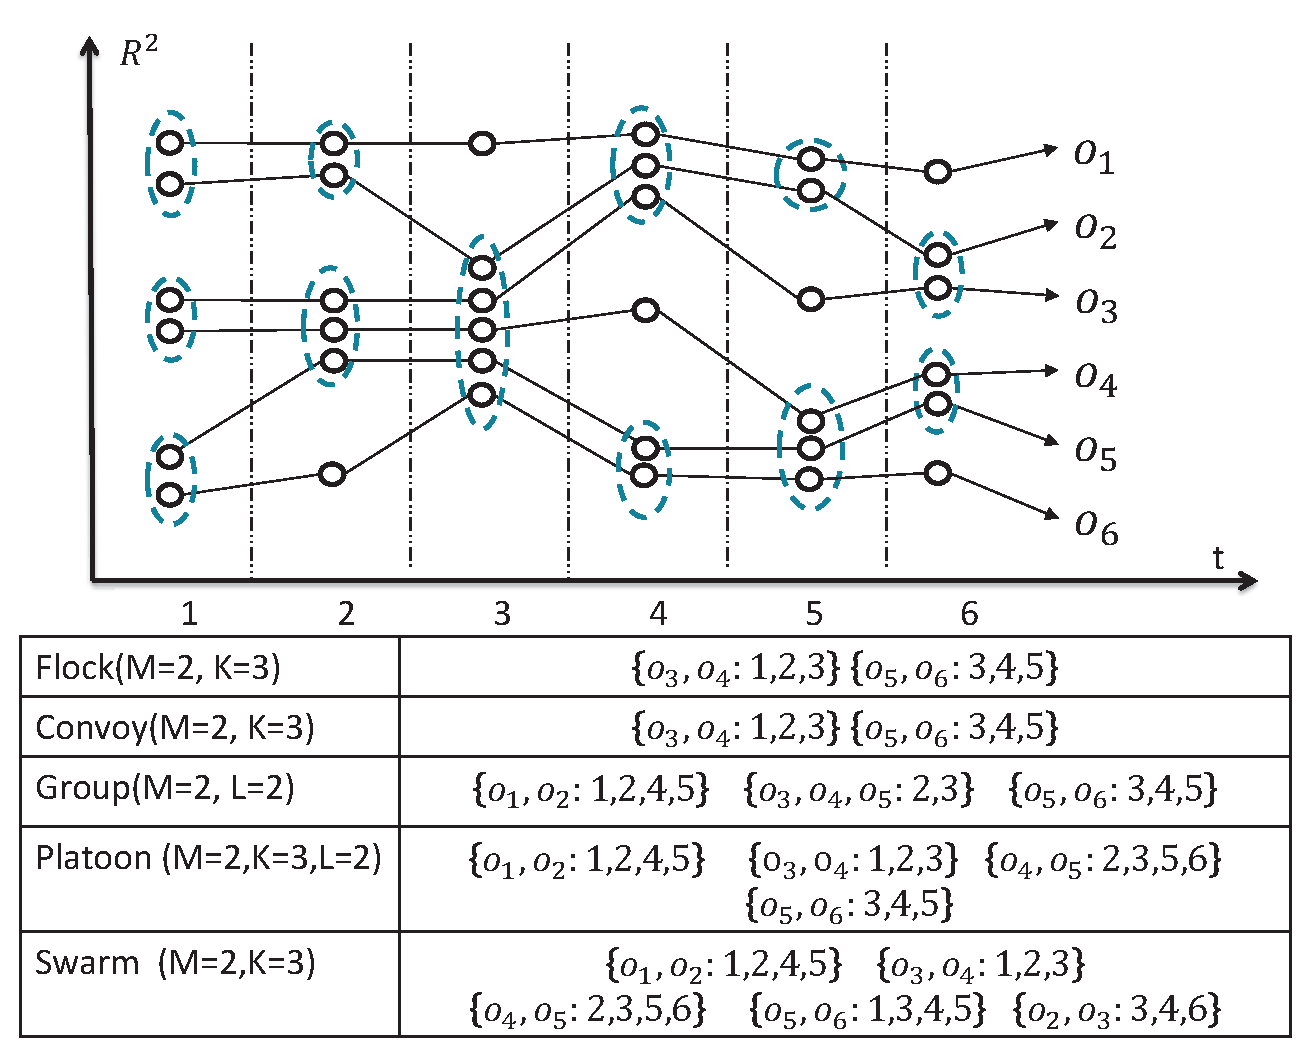
\includegraphics[width=0.45\textwidth]{related_work.eps}
\caption{Trajectories and co-movement patterns; The example consists of six trajectories across six snapshots. Objects in spatial clusters are enclosed by dotted circles. $M$ is the minimum cluster cardinality; $K$ denotes the minimum number of snapshots for the occurrence of a spatial cluster; and $L$ denotes the minimum length for local consecutiveness.}
\label{fig:related_work}
\end{figure}

Figure~\ref{fig:related_work} is an example to demonstrate the concepts of various co-movement patterns. The trajectory database consists of six moving objects and the temporal dimension is discretized into six snapshots. In each snapshot, we treat the clustering methods as a black-box and assume that they generate the same clusters. Objects in proximity are grouped in the dotted circles. As aforementioned, there are three parameters to determine the co-movement patterns and the default settings in this example are $M=2$, $K=3$ and $L=2$. Both the \emph{flock} and the \emph{convoy} require the spatial clusters to last for at least $K$ consecutive  timestamps. Hence,$\{o_3,o_4\}$ and $\{o_5,o_6\}$  remains the only two candidates matching the patterns. The \textit{swarm} relaxes the pattern matching by discarding the temporal consecutiveness constraint. Thus, it generates many more candidates than the \textit{flock} and the \textit{convoy}. The \textit{group} and the \textit{platoon} add another constraint on local consecutiveness to retain meaningful patterns. For instance, $\{o_1,o_2:1,2,4,5\}$ is a pattern matching local consecutiveness because timestamps $\{1,2\}$ and $\{4,5\}$ are two segments with length no smaller than $L=2$. The difference between the \textit{group} and the \textit{platoon} is that the \textit{platoon} has an additional parameter $K$ to specify the minimum number of snapshots for the spatial clusters. This explains why $\{o_3,o_4,o_5:2,3\}$ is a  \textit{group} pattern but not a \textit{platoon} pattern.

As can be seen, there are various co-movement patterns requested by different 
applications and it is cumbersome to design a tailored solution for each type. 
As pointed in \cite{li2015platoon, li2010swarm}, stringent temporal constraints (e.g., global consecutiveness on \emph{flock} and \emph{convoy}) may miss out many interesting patterns. However, we observe that pattern definitions with overly-relaxed temporal constraints (e.g., \emph{swarm}, \emph{group} and \emph{platoon}) lose the fine control of a pattern which introduce noisy results and unnecessary computations. We name this scenario as \emph{loose-connection} anomaly. To illustrate, as shown in Figure~\ref{fig:platoon_weakpoint}, the two objects $o_1, o_2$ form a \emph{platoon} pattern 
$\{o_1,o_2:1,2,3,102,103,104\}$. However, the consecutive segments are $98$ timestamps apart, 
making the co-moving behavior very loose.
In reality, such an anomaly is likely induced by the periodic movements of unrelated objects 
such as, vehicles stopping at the same petrol station, animals pausing at the same water source etc.  Interestingly, none of the temporal-relaxed patterns (e.g., \emph{swarm}, \emph{group} and \emph{platoon}) is able to avoid such an anomaly directly.

%In addition, existing pattern definitions are not expressive enough and may miss 
%interesting patterns or return noisy results. We summarize 
%the two scenarios as \emph{missing-pattern} anomaly
%and \emph{loose-connection} anomaly.
%A \emph{missing-pattern} anomaly arises due to the stringent constraints on the pattern duration.
%As shown in Figure~\ref{fig:platoon_weakpoint} (a), if we set $K=4$, 
%neither \emph{flock}s nor \emph{convoy}s can be discovered. This is because
%$o_1$ is away from $o_2$ at timestamp $4$, which is likely caused by
%the traffic control or the clustering inaccuracy at time $4$. On the other hand,
%the \emph{loose-connection} anomaly occurs due to an over-relaxed constraint on 
%the duration. As shown in Figure~\ref{fig:platoon_weakpoint} (b),
%the two objects $o_1, o_2$ form a \emph{platoon} pattern 
%$\{o_1,o_2:1,2,3,102,103,104\}$. However, the consecutive segments are $98$ timestamps apart, 
%making the co-moving behavior very weak.
%In reality, such an anomaly is likely to be induced by the periodic movements of unrelated objects 
%such as, vehicles stopping at the same petrol station, animals pausing at the same water source etc. 
%It is easy to see that none of the existing co-movement patterns are able to avoid these two anomalies.

\begin{figure}[h]
\center
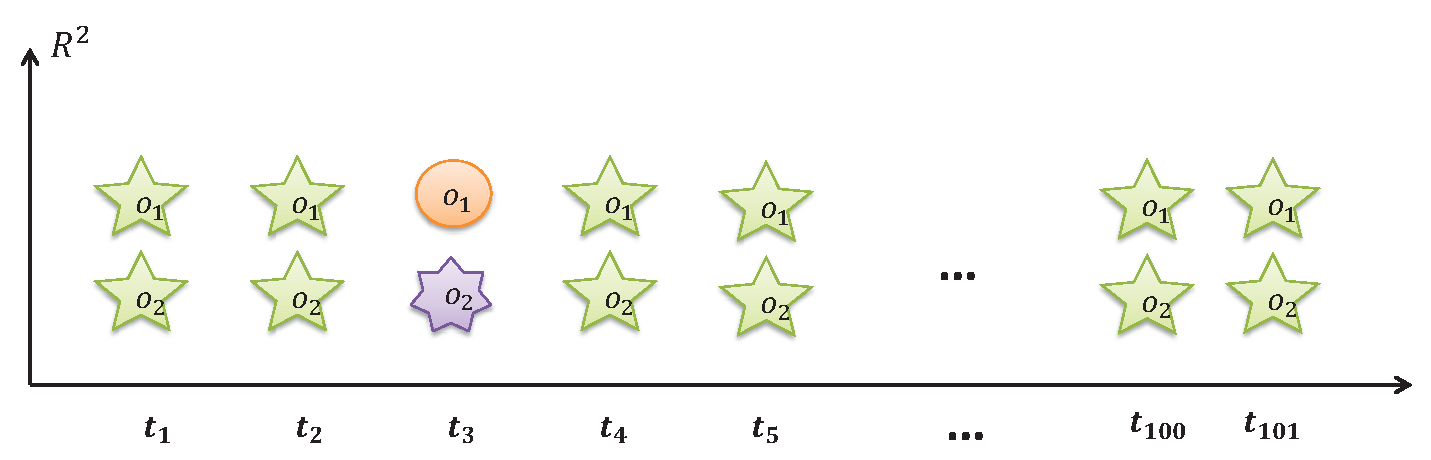
\includegraphics[width=0.35\textwidth]{platoon_weakpoint.eps}
\caption{\emph{Loose-connection} anomaly. The consecutive segment of $o_1$ and $o_2$ are 98 timestamps apart, however, the pattern $\{o_1, o_2: 1,2,3,102,103,104\}$ is included in \emph{platoon}, \emph{swarm} and \emph{group} results.}
\label{fig:platoon_weakpoint}
\end{figure}

%In current literature,
%users are unable to explicitly exclude the loosely-connected patterns even when those patterns are unwanted.
%
%
% we summarize two anomalies 
%The \emph{missing-pattern}~\cite{li2010swarm} anomaly arises due to the stringent constraints on the duration of a pattern. As shown in 
%Figure~\ref{fig:platoon_weakpoint} (a).  As we notice, object $o_1$ is temporally far from $o_2$ at timestamp $4$, which is likely to be
%the result of errors in interpretation of missing points, or $o_1$ faces traffic control at time $4$. Such an anomaly can
%be resolved by \emph{swarm} and \emph{platoon} due to a relaxed constraint on the duration. However, 
%\emph{swarm} and \emph{platoon}'s relaxations encompass a type of non-interesting patterns which is referred
%as \emph{loose-connection}~\cite{li2015platoon} anomaly. 
%
%
%%This is because that \emph{platoon} allows the timestamps in a pattern duration to be in arbitrary distance, making the object group loosely
%connected. For instance, patterns with duration $\{1,2,100,101\}$ could be a valid \emph{platoon}; however, the two timestamps $2,100$ are too far from each other.

%For instance, PUT THE FIGURE AND EXPLANATION HERE.

%\begin{figure}[h]
%\center
%\includegraphics[width=0.35\textwidth]{rw_perf_O.eps}
%\caption{Two anomalies in existing patterns. (a) \emph{Missing-pattern} anomaly
%in \emph{flock} and \emph{convoy}. When $K=4$, none of the two patterns can be discovered. (b) \emph{Loose-connection} anomaly in \emph{platoon} and \emph{swarm}. The consecutive segment of $o_1$ and $o_2$ are 98 timestamps apart, however, the pattern $\{o_1, o_2: 1,2,3,102,103,104\}$ is included in platoon and swarm results.}
%\label{fig:platoon_weakpoint}
%\end{figure}


The other issue with existing methods is that they are 
built on top of centralized indexes that are not scalable. 
To the best of our knowledge, the maximum number of trajectories 
ever evaluated is up to hundreds of trajectories. 
In practice, it is rather common to collect at least hundreds of thousands of trajectories 
and their scalability is left unknown. We conduct a theoretical analysis on the worst-case complexity (as listed in Table~\ref{tbl:existing_co_patterns}) as well as an experimental evaluation with a real trajectory database including million-scale points(as shown in Figure~\ref{fig:related_work_scalability}). 
Results show that their performances degrade dramatically as the dataset size scales up. For instances,
performance of \emph{swarm} drops five times as the number of objects grows from \emph{1k} to \emph{2k}. Similarly,
performance of \emph{group} drops over seven times as the number of snapshots grows from \emph{1.5k} to \emph{2.4k}.
It is easy to spot that none of the existing solutions are scalable to handle large-scale trajectories which may include billion-scale points.
%In fact, as shown in Table~, the mining of co-movement patterns require high complexity. For instance, the
%complexities of \emph{swarm} and \emph{platoon} are already exponential. 
%Therefore, none of them can handle millions of trajectories efficiently. 
%CAN YOU ANALYSE THEIR COMPLEXITY TO ADDRESS THE PROBLEM OF SCALABILITY.
\begin{figure}[h]
    \centering
    \begin{subfigure}[b]{0.23\textwidth}
            \centering
            \includegraphics[width=\textwidth]{rw_perf_O.eps}
		\subcaption{$1k$ objects}
    \label{fig:fig1}
    \end{subfigure}
    \begin{subfigure}[b]{0.23\textwidth}
            \centering
            \includegraphics[width=\textwidth]{rw_perf_T.eps}
         \subcaption{$1.2k$ timestamps}
    \label{fig:fig2}
    \end{subfigure}
    \caption{Performance measures on existing co-movement patterns. A sampled Geolife data set
    is used with over 2 million points.}
    \label{fig:related_work_scalability}
\end{figure}




Therefore, our primary contributions in this paper are to close these two gaps. 
First, we propose the \emph{general co-movement pattern} (GCMP) which models
various co-moment patterns in a unified way while avoids 
the \emph{loose-connection} anomaly. In GCMP, we gain a
fine-grained control over pattern duration by introducing the gap 
parameter $G$, which enforces the gap between 
timestamps to be no larger than $G$.  
The adoption of $G$ seamlessly integrates with other pattern parameters,
which preserves the expressiveness while
alleviates the \emph{loose connection} anomalies.

%Therefore, users are 
%still able to exclude non-consecutive patterns 
%or include loosely-connected patterns when they feel necessary.


%We introduce the gap parameter $G$,
%When such loosely-connected patterns are unwanted, users currently are unable to directly control the outputs.
%To cope with both of the two anomalies, we propose 
%by introducing the gap parameter $G$, 

%By so doing, we gain a fine-grained control s, which As we show in later sections, the general co-movement pattern is able to express existing patterns by setting appropriate parameters. 
%IS IT POSSIBLE TO USE FIGURE 1 TO ADDRESS THE PROBLEM OF PLATOON, INSTEAD OF PROPOSING A NEW EXAMPLE SCENARIO?
%

Second, we propose a parallel solution on modern MapReduce platforms for scalable pattern mining.
The major challenge in designing MapReduce-based algorithms is to make proper partitions of input data.
In GCMP mining, we enforce both the \emph{soundness} and the \emph{completeness} 
of the partitions. Such properties ensure that neither false-patterns 
nor miss-patterns are possible in our solution. To meet such partition requirements
as well as to keep the shuffle amount to a minimum, 
we first design a naive \emph{Temporal Replication and Mining} (TRM)
approach, which partitions trajectories into groups of consecutive snapshots. Then, we design a line-sweep
method for mining GCMP from each partition. We prove that in TRM, the partition is complete and sound when a snapshot is replicated $O(|T|)$ times. 
Then, we design a novel \emph{Star Partition and Mining} (SRM) approach which significantly reduces the data shuffled
as compare to TRM. In SRM, we design a conceptual connection graph based on proximity among objects. We adapt
a \emph{star partition} which cut the graph by replicating vertices. Afterwards, we design an Apriori-like method to mine
GCMP in each partition. We prove the correctness of SPM and show that total data been replicated is $O(|\mathbb{O}|)$. 
Despite the simpleness of star partition, we theoretically prove its optimality.
Furthermore, we utilize \emph{temporal monotonicity} to further reduce the 
shuffling and mining cost in SPM. 
%Lastly, we adapt various engineering level techniques to support efficiently deploying our algorithms in 
%Apache Spark which is one of the most popular MapReduce platforms.

%we design a novel star-based partition scheme to efficiently partition objects based on their
%belonging clusters. Based on the star partition, we then propose a series of optimization techniques which
%largely improve the system performance. NEED TO EMPHASIZE YOUR TECHNICAL CONTRIBUTION!

We conduct a set of extensive experiments on XXX datasets with million-scale trajectories. The results show that XXX.

The rest of our paper is organized as follows: Section~\ref{sec:related_works} summarizes the relevant literature on 
trajectory pattern mining; Section~\ref{sec:definition} forms the definition of the general co-movement pattern mining; Section~\ref{sec:system_overview} presents our parallel architecture; The solution of mining the general co-movement pattern mining is presented in Section~\ref{sec:trm_solution} and Section~\ref{sec:spm_solution}. Section~\ref{sec:optimization} discuss various optimization techniques to boost the system performance; Section~\ref{sec:experiment} conducts extensive experiments to showcase the usefulness and efficiency of our system and finally Section~\ref{sec:conclusion} concludes our paper.

\section{Related Work}
\label{sec:related_works}
Related work can be grouped into three categories: \emph{co-movement patterns},
\emph{dynamic movement patterns} and \emph{trajectory mining frameworks}.
%The \emph{co-movement patterns} in literature consist 
%of five members, namely \emph{group}~\cite{wang2006grouppattern}, \emph{flock}~\cite{gudmundsson2004flock},
%\emph{convoy}~\cite{jeung2008convoy}, \emph{swarm}~\cite{li2010swarm} and \emph{platoon}~\cite{li2015platoon}.
%We have demonstrated the semantics of these patterns in Table~\ref{tbl:existing_co_patterns} and Figure~\ref{fig:related_work}. 
%In this section, we distinguish the parallel GCMP mining from these concepts.
%In this section, we focus on comparing the techniques used in these works.
%For more trajectory patterns other than \emph{co-movement patterns}, 
%interested readers may move to~\cite{zheng2015survey} for a comprehensive survey.
\subsection{Co-Movement Patterns}
\subsubsection{Flock and Convoy}
The difference between \emph{flock} and \emph{convoy} lies 
in the object clustering methods. In \emph{flock},
objects are clustered based on their distances. Specifically, the
objects in the same cluster need to have a pairwise distance less than \emph{min\_dist}. 
This essentially requires the objects to be within a disk-region of delimiter less than \emph{min\_dist}.
In contrast, \emph{convoy} clusters objects using density-based spatial clustering~\cite{ester1996density}.
Technically, \emph{flock} utilizes a $m^{th}$-order Voronoi diagram~\cite{laube2005finding} to detect whether
a subset of $n$ ($n \geq m$) objects stay in a disk region.
%a subset of object with size greater than $m$ stays in a disk-region.
\emph{Convoy} employs
a trajectory simplification~\cite{douglas1973linesimplification} technique to boost pairwise distance computations in
the density-based clustering.
After clustering, both \emph{flock} and \emph{convoy} use a sequential scanning
method to examine each snapshot. 
During the scan, the object groups that do 
not appear in consecutive snapshots are pruned.
%During the scan, object
%groups that appear in consecutive timestamps are detected. Meanwhile, the object groups that do not
%match the consecutive constraint are pruned. 
However, such a method faces high complexity when supporting other patterns.
For instance, in \emph{swarm}, the candidate set during the sequential scanning grows
exponentially, and many candidates can only be pruned after the entire dataset are scanned.

\subsubsection{Group, Swarm and Platoon}
Different from \emph{flock} and \emph{convoy}, all the \emph{group},\emph{swarm} and \emph{platoon}
patterns have more relaxed constraints on the pattern duration. Therefore, their techniques of mining are of
the same skeleton. The main idea of mining is to grow an object set from an empty set
in a depth-first manner. During the growth, various pruning techniques are provided to prune 
unnecessary branches. \emph{Group} pattern uses a VG-graph to guide the pruning of false candidates~\cite{wang2006grouppattern}.
\emph{Swarm} designs two more pruning rules called backward pruning and forward pruning~\cite{li2010swarm}. \emph{Platoon}~\cite{li2015platoon}
leverages a prefix table structure to steer the depth-first search, which shows efficiency 
as compared to the other two methods.
However, the pruning rules adopted by the three patterns heavily rely on depth-first search which loses efficiency in a parallel scenario.


\subsection{Other Related Trajectory Patterns}
A closely related literature to co-movement patterns is the \emph{dynamic movement} patterns. Instead of requiring the same set of object traveling together, \emph{dynamic movement} patterns allow objects to temporally join or leave a group. Typical works include \emph{moving clusters}~\cite{kalnis2005movingclusters}, \emph{evolving convoy}~\cite{aung2010discovery}, \emph{gathering}~\cite{zheng2013gathering} etc. These works cannot model GCMP since they enforce global consecutiveness on the 
temporal domain.
 
\subsection{Trajectory Mining Frameworks}
Jinno et al. in~\cite{jinno2012paralleltpattern} designed a MapReduce based algorithm to efficiently support \emph{T}-pattern discovery, where a \emph{T}-pattern is a set of objects visiting the same place at simliar time. Li et al. proposed a framework of processing online \emph{evolving group} pattern~\cite{li2013onlinegroup}, which focuses on supporting efficient updates of arriving objects. 
As these works essentially differ from co-movement pattern, their techniques cannot be directly applied to discover GCMPs.

\section{Definitions}
\label{sec:definition}
Let $\mathbb{O} = \{o_1 ,o_2,...,o_n\}$ be the set of objects and $\mathbb{T} =\{1,2,...,m\}$ be the descritized temporal dimension. A time sequence $T$ is defined as a subset of $\mathbb{T}$, i.e., $T \subseteq \mathbb{T}$, and we use $|T|$ to denote sequence length. Let $T_i$ be $i$-th entry in $T$ and we say $T$ is consecutive if $\forall 1\leq i\leq |T|-1$, $T_{i+1} = T_i + 1$. It is obvious that any time sequence $T$ can be decomposed into consecutive segments and we say $T$ is \textit{L-consecutive}~\cite{li2015platoon} if the length of all the consecutive segments is no smaller than $L$. 

To control the closeness of timestamps, we further define the $G$-connected of a time sequence as follows: WHAT THE RELATIONSHIP BETWEEN CLOSENESS AND G-CONNECTED?


%
%
%We say a sequence $T$ is \emph{(fully)consecutive}
%if and only if $\forall T[i] \in T, T[i+1] \in T$, $T[i+1] = T[i] + 1$. A subsequence $T^m$ is \emph{maximally consecutive}~\cite{li2015platoon} wrt. $T$ if and only if $T^m \subseteq T$ and $\nexists T^{m'}, T^m \subseteq T^{m'} \wedge T^{m'} $ is consecutive. For example, let $T=\{1,2,3,5,6\}$, then $T_1=\{1,2,3\}$ and $T_2=\{5,6\}$ are two maximally consecutive subsequences wrt. $T$. We then define the $L$-consecutiveness as follows:

%\begin{definition}[$L$-consecutive~\cite{li2015platoon}]
%A time sequence $T$ is $L$-consecutive if each of its consecutive portions 
%has cardinality greater or equal to $L$.
%\end{definition}


\begin{definition}[$G$-connected]
A time sequence $T$ is $G$-connected if the gap between any of its neighboring timestamps is no greater than $G$. That is
 $\forall T[i],T[i+1] \in T, T[i+1]-T[i] \leq G$.
\end{definition}

We take $T=\{1,2,3,5,6\}$ as an example, which can be decomposed into two consecutive segments $\{1,2,3\}$ and $\{5,6\}$. $T$ is not $3$-consecutive since the length $\{5,6\}$ is $2$. Thus, it is safe to say either $T$ is $1$-consecutive or $2$-consecutive. On the other hand, $T$ is $2$-connected since the maximum gap between its neighboring time stamps is $5-3=2$. It is worth noting that $T$ is not $1$-connected because XXX.

%Given a timestamp $t$, objects with their locations at $t$ collectively form a \emph{snapshot}\footnote{Missing time stamps can be interpreted using existing methods such as linear interpolation~\cite{jeung2008convoy}.}.Objects in a snapshot can then be clustered based on the closeness of their locations. Let $C_t(o_i)$ be the cluster which $o_i$ belongs to at time $t$, a general co-movement pattern can be defined as:
Given a trajectory database descritized into snapshots, we can conduct a clustering method, either disk-based or density-based, to identify groups with spatial proximity. Let $T$ be the set of timestamps in which a group of objects $O$ are clustered. We are ready to define a more general co-movement pattern:
\begin{definition}[General Co-Movement Pattern]
A general co-movement pattern finds a set of objects $O$ satisfying the following five constraints: 1) \textit{closeness:} the objects in $O$ belong to the same cluster in the timestamps of $T$; 2) \textit{significance:} $|O| \geq M$; 3) \textit{duration:} $|T| \geq K$; 4) \textit{consecutiveness:} $T$ is L-consecutive; and 5) \textit{connection:} $T$ is $G$-connected.

%\begin{enumerate}
%\item{Closeness: $\forall o_i,o_j \in O, \forall t \in T, C_t(o_i) = C_t(o_j)$}
%\item{Significance: $|O| \geq M$}
%\item{Duration: $|T| \geq K$}
%\item{Consecutiveness: $T$ is $L$-consecutive}
%\item{Separateness: $T$ is $G$-separated}
%\end{enumerate} 
\end{definition}
There are XXX parameters in our general co-movement pattern, including XXX. By customizing these parameters, our pattern can be reduced to the patterns proposed in previous literature, as illustrated in Table~\ref{tbl:patterns}. In particular, by setting $G=|T|$, we achieve the \emph{platoon} pattern. By setting $G=|T|,L=1$, we achieve the \emph{swarm} pattern. By setting $G=|T|$, $M=2$, $K=1$, we gain the \emph{group} pattern. Finally by setting $G=1$, we achieve the \emph{convoy} and \emph{flock} pattern. 
In addition to covering existing patterns, the general co-movement pattern avoids the \emph{loose connection} problem in \emph{platoon} pattern. As suggested previously, $\{1,2, 100,101\}$ will be included in the platoon pattern, however since they're too far away, this pattern is not prominent. By setting appropriate $G$, we are able to prune this anomaly. It is notable that GCMP is not able to be modeled by existing patterns. AS MENTIONED IN WECHAT, POLISH THIS PART.

%The general co-movement pattern retains the patterns that discovered by all 
%existing techniques (group, flock, convoy, swarm and platoon). 
%The relationships between general co-movement pattern and other patterns are summarized 
\begin{table}
\centering
\begin{tabular}{|c|c|c|c|c|}
\hline 
Pattern & $L$ & $G$ & $M$ & $K$ \\ 
\hline
Group & $\cdot$ & $|T|$ & $2$ & $1$ \\
\hline
Flock & $K$ & 1 & $\cdot$ & $\cdot$ \\
\hline 
Convoy & $K$ & $1$ & $\cdot$ & $\cdot$\\ 
\hline 
Swarm & $1$ & $|T|$ & $\cdot$ & $\cdot$ \\ 
\hline 
Platoon & $\cdot$ & $|T|$ & $\cdot$ & $\cdot$\\ 
\hline 
\end{tabular} 
\caption{Representing other patterns using GCMP. $\cdot$ means user specified value.}
\label{tbl:patterns}
\end{table}
 
It is also observable that the number of patterns in GCMP is exponential. To control the size of output, 
we notice that, for two patterns $P_1,P_2$, if $P_1.O \subseteq P_2.O$ and $P_2$ is a proper pattern, then $P_1$ is also a proper pattern. Therefore, we can define the \emph{Closed General Co-Movement Pattern} as follows:

\begin{definition}[Closed General Co-Movement Pattern]
A general co-moving pattern $P=\langle O, T \rangle$ is closed if and only if there does not exist another general co-moving pattern $P'$ s.t. $P.O \subseteq P'.O$.
\end{definition}

For example, let $n=2,k=2,l=1,g=1$, the pattern $\{o_1,o_2\}\{1,2,3,4\}$ is not a closed pattern, while $\{o_1,o_2,o_3\}$ $\{1,2,3,4\}$ is a closed pattern. The closed pattern avoids outputting duplicate information, thus making the result patterns more compact. 

LETS KEEP THE CLOSED INFORMATION AT THE MOMENT. IF NO CLOSED IS DEFINED, WE CANNOT REDUCE GCMP TO OTHER PATTERNS SINCE THOSE PATTERNS ARE ALL DEFINED AS ``CLOSED''
%For example, let $n=2,k=2,l=1,g=1$, the pattern $\{o_3,o_4\} \{1,2,3\}$ in Figure~\ref{fig:related_work} is not a closed pattern, while $\{o_3, o_4\} \{t_1,t_2,t_3\}$ is a closed pattern. 

%Although the general co-moving pattern is free from the clustering methods used at each snapshot, as suggested in~\cite{jeung2008convoy}, the \emph{density}-based clustering method is better in detecting object clusters with arbitrary spatio-shapes. Therefore in this paper, we mainly consider density-based clustering.
Our definition of GCMP is free from clustering method. Users are able to supply different clustering method to facilitate different needs. We currently expose both disk-region based clustering and DBSCAN as options to the user.

In summary, the goal of this paper is to present a parallel solution for discovering closed GCMP from large-scale trajectory data.

Before we move on to the algorithmic part, we list the notations that are used in the following sections.

\begin{table}[h]
\centering
\begin{tabular}{|c|c|} 
\hline
Symbols & Meanings \\
\hline 
$Tr_i$ & Trajectory of object $i$\\ 
\hline
$S_t$ & Snapshot of objects at time $t$ \\
\hline 
$\mathbb{O}$ & Set of objects \\ 
\hline 
$T$ & Time sequence \\
\hline
$C_t(o)$ & the cluster of object $o$ at time $t$ \\
\hline 
$Sr_i $ &  The star structure of object $i$ \\
\hline 
\end{tabular} 
\caption{Notions that will be used}
\end{table}


\begin{figure*} [t]
\center
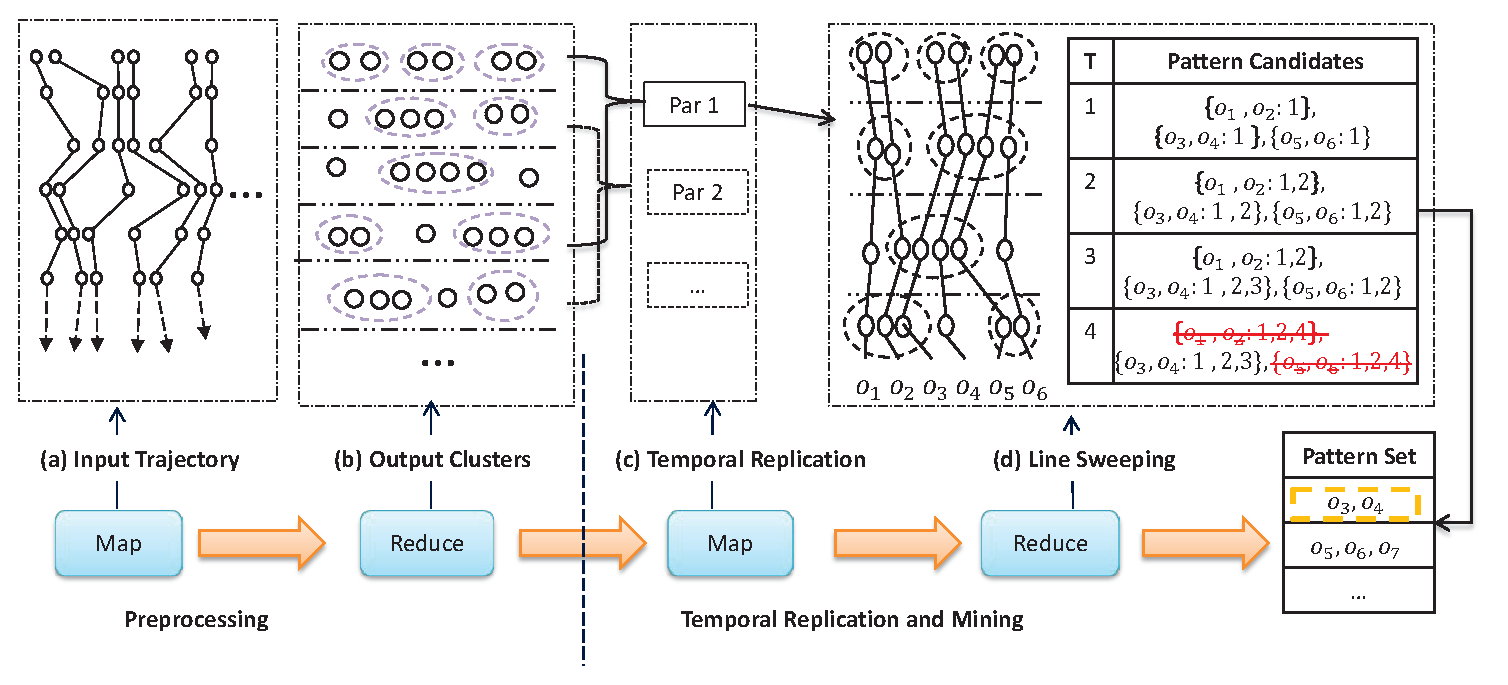
\includegraphics[width=\textwidth]{trm.eps}
\caption{Work flow of Temporal Replication and Parallel Mining. (a)(b) correspond to the first map-reduce cycle which clusters objects in each snapshot;  (c)(d) correspond to the second map-reduce cycle uses TRPM to detect GCMP in parallel.}
\label{fig:trm}
\end{figure*}

\section{Baseline: Temporal Replication and Parallel Mining}
\label{sec:trm}
In this section, we propose a baseline solution that resorts to MapReduce (MR) as a general, parallel and scalable paradigm for GCMP pattern mining. The framework, named \textit{temporal replication and parallel mining} (TRPM), is illustrated in   Figure~\ref{fig:trm}. There are two cycles of map-reduce jobs connected in a pipeline manner. The first cycle deals with spatial clustering in each snapshot, which can be seen as a preprocessing step for the subsequent pattern mining. In particular, the timestamp is treated as the key in the map phase and objects within the same snapshot are clustered (DBSCAN or disk-based clustering) in the reduce phase. Finally, the reducers output clusters of objects in each snapshot, represented by a list of key-value pairs $\langle t, S_t  \rangle$, where $t$ is the timestamp and $S_t$ is a set of clustered objects at snapshot $t$. 

Our focus in this paper is the second map-reduce cycle of parallel mining, which essentially consists of two key questions to solve. The first is how to employ effective data partitioning such that the mining can be conducted independently; and the second is how to efficiently mine the valid patterns within each partition. 


It is obvious that we cannot simply split the trajectory database 
into disjoint partitions because a GCMP pattern requires $L$-consecutiveness 
and the corresponding segments may cross multiple partitions. 
Our strategy is to use data replication to enable parallel mining. 
Each snapshot will replicate its clusters to $\eta-1$ preceding snapshots.
In other words, the partition for the snapshot $S_t$ contains clusters 
in $S_t$, $S_{t+1}\ldots,S_{t+\eta-1}$. 
Determining a proper $\eta$ is critical in ensuring the
correctness and efficiency of TRPM. If $\eta$ is too small, 
certain cross-partition patterns may be missed. 
If $\eta$ is set too large, expensive network communication and 
CPU processing costs would be incurred in the map and reduce phases respectively. Our objective is to find an $\eta$ that is not large but can guarantee correctness.


In our implementation, we set $\eta = (\lceil \frac{K}{L} \rceil - 1)*(G-1)+K+L-1$. Intuitively, $K$ timestamps generates at most $\lceil \frac{K}{L} \rceil - 1$ gaps as the length of each $L$-consecutive segment is at least $L$. Since the gap size is at most $G-1$, $(\lceil \frac{K}{L} \rceil - 1)*(G-1)$ is the upper bound of timestamps allocated to gaps. The remaining part $K+L-1$ is used to capture the upper bound allocated for the $L$-consecutive segments. We formally prove that $\eta$ can guarantee correctness.


\eat{
Before moving on to find the value of $\eta$, 
we first use $\rho_{G,L,K}(T)$ to define the \emph{min-spanned valid subsequence} 
of a sequence $T$. In simple words, $\rho_{G,L,K}(T)$ is the 
subsequence of $T$ with the smallest range and is valid wrt. $K,L,G$. 
%Let $\eta_T$ denote
%the range of $\rho_{G,L,K}(T)$.
To guarantee that no valid patterns are missing, $\eta$ needs
to be greater than the range of $\rho_{G,L,K}(T)$ for any
valid sequence $T$. To see this, consider an arbitrary valid sequence $T$.
Since each partition contains $\eta$ snapshots,
if $\eta \geq \range(\rho_{G,L,K}(T))$ holds, $\rho_{G,L,K}(T)$ must be completely located in one partition. Therefore, the patterns associated with $T$ would not be missing.
Formally, $\eta$ can be computed as:
\begin{equation}
\eta = \max\{\range(\rho_{G,L,K}(T)) | T \text{ is valid wrt. } G,L,K\}
\end{equation}

Directly compute such $\eta$ is challenging. However,
we provide the following theorem which states a bounded estimation on $\eta$: 
}



\begin{theorem}
\label{THM:RP_ETA}
$\eta = (\lceil \frac{K}{L} \rceil - 1)*(G-1)+K+L-1$ guarantees that no valid pattern is missing.
\end{theorem}
\begin{proof}
Given a valid pattern $P$, we can always find at least one valid subsequence that is also valid. Let $T'$ denote the valid subsequence with the minimum length. In the worst case, $T'=P.T$. We define $\range(T)=\max(T) - \min(T) +1$ and prove the theorem by showing that $\range(T') \leq \eta$.
Since $T'$ can be written as a sequence of L-consecutive segments interleaved by gaps: $l_1,g_1,\ldots,l_{n-1},g_{n-1},l_n$ ($n \geq 1$),
where $l_i$ is a segment and $g_i$ is a gap. Then, $\range(T')$
is calculated as $\Sigma_{i=1}^{i=n}|l_i| + \Sigma_{i=1}^{i=n-1} |g_i|$. Since $T'$
is valid, then $\Sigma_{i=1}^{i=n}|l_i| \geq K$. As $T'$ is minimum, if we remove the 
last $l_n$, the resulting sequence should not be valid. Let $K' = \Sigma_{i=1}^{i=n-1}|l_i|$, which
is the size of the first $(n-1)$ segments of $T'$. Then, $K' \leq K-1$.
Note that every $|l_i| \geq L$, thus $n \leq \lceil \frac{K'}{L} \rceil \leq \lceil \frac{K}{L} \rceil $. By
using the fact that every $|g_i| \leq G-1$, we achieve $\Sigma_{i=1}^{i=n-1} |g_i| \leq (n-1)(G-1)
\leq (\lceil \frac{K}{L} \rceil -1)(G-1)$. Next, we consider the difference between $K$ and $K'$, denoted by
$\Delta = K- K'$. To ensure $T'$'s validity, $l_n$ must equal to $\min(L, \Delta)$.
Then, $\Sigma_{i=1}^{i=n}|l_i| = K' + l_n = K - \Delta + \min(L, \Delta) \leq K - 1 + L$. We finish showing $\range(T') \leq \eta$.  Therefore, for any valid sequence $T$, it exists at least one valid subsequence with range no greater than $\eta$ and hence this pattern can be detected in a partition with $\eta$ snapshots.
\end{proof}

\eat{
Note that Theorem~\ref{THM:RP_ETA} does not state the optimal value of $\eta$
for a given $G,L,K$. However, for any $G,L,K$, $\eta$ does not differ from
the optimal value by at most $L-1$. To see this, for any $G,L,K$, we can
generate a sequence $T$ by repeating the following pattern, a $L$-segment followed by $G$-gap. 
The repetition stops when $|T|\geq K$. Apparently $T$ is valid wrt. $G,L,K$.
It is easy to see that $T$ is minimal valid subsequence of itself, then $\eta^*  \geq \range(T) \geq (\lceil \frac{K}{L}\rceil -1)(G-1) + K$.
Therefore $\eta-\eta^* \leq L-1$.
}

\begin{algorithm}[h]
\caption{Line Sweep Mining}
\label{algo:line-sweep}
\begin{algorithmic}[1]
\Require $\lambda_t = \{S_t, ..., S_{t+\eta-1}\}$
\State{$C \gets \{\}$} \Comment{Candidate set} \label{code:ls-can-set}
\ForAll{clusters $s$ in snapshot $S_t$} 
\label{code:ls-init-start}
\If{$|s| \geq M$}
\State $C\leftarrow C\cup \{\langle s, t \rangle \}$
\EndIf
\EndFor
\label{code:ls-init-end}
\ForAll{$S_j \in \{S_{t+1},\ldots,S_{t+\eta-1}\}$} \label{code:ls-sweep-starts}
	\State $N \gets \{\}$
	\ForAll {$(c,s) \in C \times S_j$} \label{code:ls-join-start}
		\State {$c' \gets \langle c.O \cap s.O, c.T \cup \{j\} \rangle$} \label{code:ls-join}
		\If {$c'.T$ is valid} 
			\State output $c'$
		\ElsIf{$|c'.O| \geq M$}
			\State $N\leftarrow N\cup \{c'\}$ \label{code:ls-m-prun}	
		\EndIf
	\EndFor \label{code:ls-join-ends}
	\ForAll {$c \in C$}
		\If{$j-\max(c.T)\geq G$}\label{code:ls-g-prune-starts}
			\State $C\leftarrow C-\{c\}$ 
			\State output $c$, if $c$ is a valid pattern
		\EndIf  \label{code:ls-g-prune-ends}
		\If{$c$'s first segment is less than $L$}\label{code:ls-l-prune-starts}
			\State $C\leftarrow C-\{c\}$ 
		\EndIf\label{code:ls-l-prune-ends}
	\EndFor
	\State $C\leftarrow C\cup N$
\EndFor\label{code:ls-sweep-ends}
\State output valid patterns in  $C$  \label{code:ls-valid-check}
\end{algorithmic}
\end{algorithm}



Based on the above theorem, during TRPM, every consecutive $\eta$ snapshots
form a partition. In other words, each snapshot $S_t$ corresponds to a partition $\lambda_t=\{S_t,...,S_{t+\eta-1}\}$. Our next task is to design an efficient pattern mining strategy within each partition. We propose a line sweep algorithm to sequentially scan the $\eta$ replicated snapshots in a partition and employ effective candidate pattern enumeration.  

Details of the algorithm are presented in Algorithm~\ref{algo:line-sweep}. We keep a candidate set $C$ (Line~\ref{code:ls-can-set}) during the sweeping process. It is initialized as the candidate clusters with size no smaller than $M$ in the first snapshot. Then, we sequentially scan each snapshot (Lines~\ref{code:ls-sweep-starts}-\ref{code:ls-sweep-ends}) and generate new candidates by extending the original ones in $C$.
In particular, we join candidates in $C$ with all the clusters in $S_j$ to form new candidates (Lines~\ref{code:ls-join-start}-\ref{code:ls-join-ends}). 
%The join of candidate $c$ and cluster $s$ creates a
%new candidate $c'$ (Line~\ref{code:ls-join}).  
After sweeping all the snapshots, all the valid patterns are stored in $C$(Line~\ref{code:ls-valid-check}). 
It is worth noting that $C$ continues to grow during the whole sweeping process. We can use three pruning rules to 
early remove false candidates from $C$. Since there is a partition $\lambda_t$ for each $S_t$, only patterns that start from timestamp $t$ need to be discovered. Therefore, those patterns that does not appear in the $S_t$ are false candidates. Particularly, our
three pruning rules are as follows:
First, when sweeping snapshot $S_j$, new candidates with objects set smaller than $M$ are pruned (Line~\ref{code:ls-m-prun}). Second, after joined with all clusters in $S_j$, 
candidates in $C$ with the maximum timestamp no greater than $j-G$ are pruned (Lines~\ref{code:ls-g-prune-starts}-\ref{code:ls-g-prune-ends}). Third, candidates in $C$ with the size of first segment smaller than $L$
are pruned (Lines~\ref{code:ls-l-prune-starts}-\ref{code:ls-l-prune-ends}). With the three pruning rules, the size of $C$ could be significantly reduced.  

%ADD EXPLANATIONS TO THE SECOND AND THIRD PRUNING RULES.

%After join, there are two prunings. First, 
%all new candidates with objects set less than $M$ are pruned (Line~\ref{code:ls-m-prun}). Second,
%existing candidates with max time sequences no greater 
%than $j-G$ are pruned (Line~\ref{code:ls-m-prun}). 
% 
%
%During the sweeping, candidates in $\mathbf{C}$ join with $S_j$.
%
% Initially, all the clusters 
%
%During scanning, a set of pattern candidates is maintained.
%When all snapshots are scanned, the remaining candidates are the true patterns.
%The detail of LSM is presented in Algorithm~\ref{algo:line-sweep}.
%A candidate set $C$ is maintained throughout the algorithm(line~\ref{code:ls-can-set}). $C$
%is initialized by inserting clusters at $S_t$ (lines~\ref{code:ls-init-start}-\ref{code:ls-init-end}).
%During scanning snapshot $S_j$, candidates in $C$ are joined with clusters at $S_j$. In
%the join, a candidate grows its temporal sequence while potentially reduces its object set. After the join,
%false patterns are deleted (line~\ref{code:ls-remove}). 
%Note that the size of $C$ is always decreasing, therefore the complexity of LSM $\lambda_t$ is $O(\eta|S_t||\overline{S}|)$,where $|\overline{S}|$ is the average snapshot size in $\lambda_t$.

The complete picture of temporal replication and parallel mining is summarized in Algorithm~\ref{algo:trm_overview}. We illustrate the workflow of TRPM method using Figure~\ref{fig:trm} (c)(d) with pattern
parameters $M=2, K=3, L = 2, G=2$. By Theorem~\ref{THM:RP_ETA}, $\eta$ is calculated
as $(\lceil \frac{K}{L} \rceil-1) *(G-1)+2K - 2 = 5$. Therefore, 
in Figure~\ref{fig:trm} (c), every $5$ consecutive snapshots are combined 
into a partition in the map phase. In Figure~\ref{fig:trm} (d), a line sweep
method is illustrated for partition $\lambda_1$. Let $C_i$ be the candidate set
during sweeping snapshot $S_i$.
Initially, $C_1$ contains patterns with object sets in snapshot $S_1$.
As we sweep the snapshots, the patterns in $C_i$ grow. At snapshot $S_4$, the candidate
$\langle o_5,o_6 \rangle$ is removed. This is because the gap between its latest timestamp (i.e., $2$)
and the next scanning timestamp (i.e., $5$) is $3$, which violates the $G$-connected constraint.
Next, at snapshot $S_5$, the candidate $\langle o_1,o_2 \rangle$ is removed. This is
because its local consecutive segment $(4)$ has only $1$ element,
which violates the $L$-consecutive constraint.
Finally, $\langle o_3,o_4 \rangle$ is the valid pattern and is returned. Note that in this example, $\eta=5$ is the minimum setting that can guarantee correctness. If $\eta$ is set to $4$, the pattern $\langle o_3,o_4 \rangle$ would be missed. 

\begin{algorithm}[h]
\caption{Temporal Replication and Parallel Mining}
\label{algo:trm_overview}
\begin{algorithmic}[1]
\Require list of $\langle t, S_t \rangle$ pairs
\State $\eta \gets (\lceil \frac{K}{L} \rceil -1)*(G-1)+K+L-1$
\State {---Map Phase---}
\label{code:trm-map-start}
\ForAll{snapshots $S_t$}
	\ForAll{$i \in 1...{\eta-1}$}
		\State emit key-value pair $\langle \max(t-i,0), S_t \rangle$ 
	\EndFor  
\EndFor
\label{code:trm-map-end}
\State {---Partition and Shuffle Phase---}
\label{code:trm-par-start}
\ForAll{key-value pairs $\langle t, S \rangle$ pair} 
\State group-by $t$ and emit a key-value pair $\langle t, \lambda_t\rangle$, where $\lambda_t = \{S_t, S_{t+1}, .. S_{t+\eta-1}\} $
\EndFor
\label{code:trm-par-end}
\State {---Reduce Phase---}
\label{code:trm-red-start}
\ForAll{key-value pairs $\langle t,\lambda_t \rangle$}
\State call line sweep algorithm for partition $\lambda_t$
\label{code:trm-red-end}
\EndFor
\end{algorithmic}
\end{algorithm}

\begin{figure*}[t]
\centering
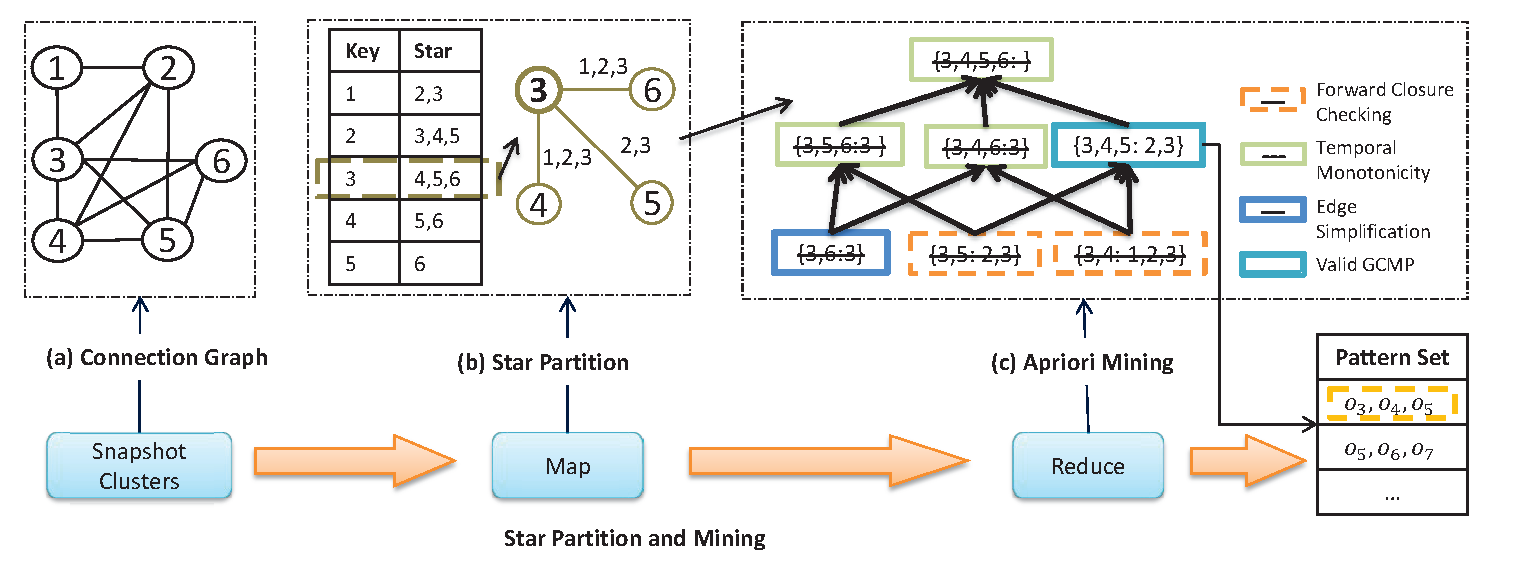
\includegraphics[width=0.9\textwidth]{spm.eps}
\caption{Star partition and ApRiori Enumerator (SPARE). (a) Aggregate graph from Figure 1. (b) Five stars are generated, star IDs are circled, the vertexes and inverted lists are in the connected tables.
(c) Apriori Enumerator with various pruning techniques.}
\label{fig:star_partition}
\end{figure*}

\section{SPARE: Star Partitioning and Apriori Enumerator}
\label{sec:spm}
The aforementioned replicate partitioning is based on the temporal dimension which suffers from two drawbacks. First, the replication relies on $\eta$ which could be large. Second, the same valid pattern may be discovered from different partitions which results in redundant works.
To resolve the limitations caused by the replicate partitioning, 
we propose a new Star Partitioning and ApRiori Enumerator, named SPARE, 
to replace the second cycle of map-reduce jobs in Figure~\ref{fig:trm}. 
Our new parallel mining framework is shown in Figure~\ref{fig:star_partition}. 
Its input is the set of clusters generated in each snapshot and the output 
contains all the valid GCMP patterns. In the following, we explain the two major components: 
star partitioning and apriori enumerator.


\subsection{Star Partitioning}
Let $G_t$ be a graph for snapshot $S_t$, in which each node 
is a moving object and two objects are connected if they appear 
in the same cluster. It is obvious that $G_t$ consists of a set of small cliques. 
Based on $G_t$, we define an aggregated graph $G_A$ to summarize the 
cluster relationship among all the snapshots. In $G_A$, two objects
form an edge if they are connected in any $G_t$s. Furthermore, 
we attach an inverted list for each edge, 
storing the associated timestamps in which the two objects are connected. 
An example of $G_A$, built on the trajectory database in Figure~\ref{fig:related_work}, 
is shown in Figure~\ref{fig:star_partition} (a). 
As long as two objects are clustered in any timestamps, they are connected in $G_A$. 
The object pair $\langle o_1,o_2 \rangle$ appears in two clusters at timestamps 
$2$ and $3$ and is thus associated with an inverted list $(2,3)$.


We use \emph{star} as the data structure to capture the pair relationships. 
To avoid duplication, as $G_t$ is an undirected graph and an edge may appear in multiple stars, 
we enforce a global ordering among the objects and propose a concept named \textit{directed star}.

\begin{definition}[Directed Star]
Given a vertex with global id $s$, its directed star $Sr_s$ is defined as the set of neighboring vertices with global id $t>s$. We call $s$ the star ID.
\end{definition}

With the global ordering, we can guarantee that each edge is contained in a unique star partition. Given the aggregated graph $G_A$  in Figure~\ref{fig:star_partition} (a), we enumerate all the possible directed stars in Figure~\ref{fig:star_partition} (b). These stars are emitted from mappers to different reducers. The key is the star ID and the value is the neighbors in the star as well as the associated inverted lists. 
The reducer will then call the Apriori-based algorithm to enumerate all the valid GCMP patterns.


Before we introduce the Apriori enumerator, we are interested to 
examine the issue of global ordering on the moving objects.
This is because assigning different IDs to the objects will result in 
different star partitioning results, which will eventually affect the workload 
balance among the map-reduce jobs. The job incurring performance bottleneck is often known as \emph{straggler}~\cite{kwon2012skewtune,xin2013shark,coppa2015data}. In the context of star partitioning, a straggler refers to the job assigned with the maximum star partition. We use $\Gamma$ to denote the size of a partition and $\Gamma$ is set to the number of edges in a directed star\footnote{A star is essentially a tree structure and the number of nodes equals the number of edges minus one.}. It is straightforward that a star partitioning with small $\Gamma$ is preferred. For example, Figure~\ref{fig:star-alt} gives two star partitioning results under 
different vertex ordering on the same graph. The top one has $\Gamma = 5$ while the bottom one has $\Gamma = 3$. Obviously, the bottom one with smaller $\Gamma$ is much more balanced.

\begin{figure}[h]
\centering
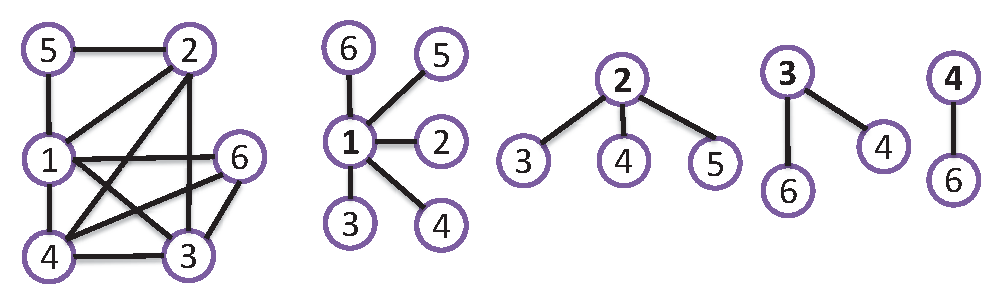
\includegraphics[width=0.5\textwidth]{star-alt.eps}
\caption{Examples of star partitioning with different vertex ordering.}
\label{fig:star-alt}
\end{figure}

Although it is very challenging to find the optimal vertex id ordering from the $n!$ possibilities, we observe that a random order can actually achieve satisfactory performance based on the following theorem.


\begin{theorem}
\label{THM:SPM_LB}
Let $\Gamma^*$ be the value derived from the optimal vertex ordering and  $\Gamma$ be value derived from a random vertex ordering. With probability $1-1/n$, we have $\Gamma = \Gamma^* + O(\sqrt{n \log n})$.
\end{theorem}
\begin{proof}
In Appendix~\ref{apx:thm2proof}.
\end{proof}
If $G_A$ is a dense graph, we can get a tighter bound for $(\Gamma - \Gamma^*)$.
\begin{theorem}
\label{THM:SPM_LB_INC}
Let $d$ be the average degree in $G_A$. If $d\geq \sqrt{12\log n}$, with
high probability $1-1/n$, $\Gamma = \Gamma^* + O(\sqrt{d\log n})$.
\end{theorem}
\begin{proof}
In Appendix~\ref{apx:thm2proof}.
\end{proof}
Hence, we can simply use object id to determine the vertex ordering in our implementation.


\subsection{Apriori Enumerator}
Intuitively, given a GCMP pattern with an object set $\{o_1,o_2,\ldots,o_m\}$, 
all the pairs of $\langle o_i,o_j \rangle$ with $1\leq i<j\leq m$ must 
be connected in the associated temporal graphs $\{G_t\}$. This inspires us to leverage the classic Apriori algorithm to enumerate all the valid GCMP patterns starting from pairs of objects. However, we observe that the monotonicity property does not hold between an object set and its supersets.

\begin{example}
In this example, we show that if an object set is not a valid pattern, we cannot prune all its super sets.
Consider two candidates $P_1=\langle o_1,o_2:1,2,3,6 \rangle$ and $P_2=\langle o_1,o_3:1,2,3,7 \rangle$. 
Let $L=2,K=3$ and $G=2$. Both candidates are not valid patterns because the constraint on $L$ is not satisfied. 
However, when considering their object superset $\langle o_1,o_2,o_3 \rangle$, we can infer that their co-clustering timestamps are in $(1,2,3)$. This is a valid pattern conforming to the constraints of $L,K,G$. Thus, we need a new type of monotonicity to facilitate pruning.
\end{example}   


\subsubsection{Monotonicity}
To ensure the monotonicity, we first introduce a procedure named \textit{star simplification}, to reduce the number of edges as well as unnecessary timestamps in the inverted lists. For instance, if the size of the inverted list for an edge $e$ is smaller than $K$, then the edge can be safely removed because the number of timestamps in which its supersets are clustered must also be smaller than $K$. To generalize the idea, we propose three concepts named \textit{maximal $G$-connected subsequence}, \emph{decomposable sequence} and \emph{sequence simplification}.

\begin{definition}[Maximal $G$-connected Subsequence]
A sequence $T'$ is said to be a maximal $G$-connected subsequence of $T$ if (1) $T'$ is the subsequence of $T$, i.e., $\exists i\leq j, T' = T(i,\ldots,j)$ , (2) $T'$ is $G$-connected, and (3) there exists no other subsequence $T''$ of $T$ such that $T'$ is the subsequence of $T''$ and $T''$ is G-connected.
\end{definition}

\begin{example}
Suppose $G=2$ and consider two sequences $T_1=(1,2,4,5,6,9,10,11,13)$ and $T_2=(1,2,4,5,6,8,9)$. $T_1$ has two maximal $2$-connected subsequences:$T_1^A=(1,2,4,5,6)$ and $T_1^B=(9,10,11,13)$. This is because the gap between $T_1^A$ and $T_1^B$ is $3$ and it is impossible for the timestamps from  $T_1^A$ and $T_1^B$ to form a new subsequence with $G\leq 2$. Since $T_2$ is $2$-connected, $T_2$ has only one maximal $2$-connected subsequence which is
itself. 
\end{example}

The maximal $G$-connected subsequence has the following two properties:
\begin{lemma}\label{lemma:union-property}
Suppose $\{T_1,T_2,\ldots,T_m\}$ is the set of all maximal $G$-connected subsequences of $T$, we have (1) $T_i\cap T_j=\emptyset$ for $i\neq j$ and (2) $T_1\cup T_2\cup\ldots\cup T_m=T$.
\end{lemma}
\begin{proof}
We assume $T_i\cap T_j\neq \emptyset$. Let $T_i=(T_i[1], T_i[2],\ldots,T_i[p])$ and $T_j= (T_j[1], T_j[2],\ldots,T_j[n])$. Suppose $T[x]$ is a timestamp occurring in both $T_i$ and $T_j$. Let $T[y]=\min\{T_i[1],T_j[1]\}$, i.e., the minimum timestamp of $T_i[1]$ and $T_j[1]$ occurs at the $y$-th position of sequence $T$. Similarly, we assume $T[z]=\max\{T_i[p], T_j[n]\}$. Apparently, the two subsequences $T[y:x]$ and $T[x:z]$ are $G$-connected because $T_i$ and $T_j$ are both $G$-connected. Then, sequence $(T_y,\ldots,T_x,\ldots,T_z)$, the superset of $T_i$ and $T_j$, is also $G$-connected. This contradicts with the assumptions that $T_i$ and $T_j$ are maximal $G$-connected subsequences. 




To prove (2), we assume $\cup_i T_i$ does not cover all the timestamps in $T$. Then, we can find a subsequence $T'=T[x:x+t]$ such that $T[x-1]\in T_a$ $(1\leq a\leq m)$, $T[x+t+1]\in T_b$ $(1\leq b\leq m)$ and all the timestamps in $T'$ is not included in any $T_i$. Let $g'=\min\{T[x]-T[x-1], T[x+t+1]-T[x+t]\}$. If $g'\leq G$, then it is easy to infer that $T_a$ or $T_b$ is not a maximal $G$-connected subsequence because we can combine it with $T[x]$ or $T[x+t]$  to a form superset which is also $G$-connected. If $g'>G$, $T'$ itself is a maximal $G$-connected subsequence which is missed in $\cup T_i$. Both cases lead to contradiction.
\end{proof}




\begin{lemma}\label{lemma:subset-property}
If $T_1$ is a subset of $T_2$, then for any maximal $G$-connected subsequence $T_1'$ of $T_1$, we can find a maximal $G$-connected subsequence $T_2'$ of $T_2$ such that $T_1'$ is a subset of $T_2'$.
\end{lemma}
\begin{proof}
Since $T_1' \subseteq T_1 \subseteq T_2 $, we know $T_1'$ is a $G$-connected subsequence of $T_2$. Based on Lemma~\ref{lemma:union-property}, we can find a maximal $G$-connected subsequence of $T_2$, denoted by $T_2'$, such that $T_1'\cap T_2'\neq \emptyset$. If there exists a timestamp $T_1'[x]$ such that $T_1'[x]\notin T_2'$, similar to the proof of case (1) in Lemma~\ref{lemma:union-property}, we can obtain a contradiction. Thus, all the timestamps in $T_1'$ must occur in $T_2'$.
\end{proof}

\begin{definition}[Decomposable Sequence]
$T$ is decomposable if for any of its maximal $G$-connected subsequence $T'$, we have (1) $T'$ is $L$-consecutive; and (2) $|T'|\geq K$.
\end{definition}

\begin{example}
Let $L = 2, K = 4$ and we follow the above example. $T_1$ is not a decomposable sequence
because one of its maximal $2$-connected subsequence (i.e., $T_1^B$) is not $2$-consecutive.
In contrast, $T_2$ is a decomposable sequence because the sequence itself is the maximal $2$-connected subsequence, which is also $2$-consecutive and with size no smaller than than $4$.
\end{example}

\begin{definition}[Sequence Simplification]
Given a sequence $T$, the simplification procedure $\mathtt{sim}(T) =  g_{G,K} \cdot f_L(T) $ can be seen as a composite function with two steps: 
\begin{enumerate}
\item $f$-step: remove segments of $T$ that are not $L$-consecutive;
\item $g$-step: among the maximal $G$-connected subsequences of $f_L(T)$, remove those with size smaller than $K$.
\end{enumerate}
\end{definition}


\begin{example}
Take $T=(1,2,4,5,6,9,10,11,13)$ as an example for sequence simplification. 
Let $L = 2, K = 4$ and $G = 2$. In the $f$-step, $T$ is reduced to $f_2(T)=(1,2,4,5,6,9,10,11)$. 
The segment $(13)$ is removed due to the constraint of $L=2$. 
$f_2(T)$ has two maximal $2$-consecutive subsequences: $(1,2,4,5,6)$ and $(9,10,11)$. 
Since $K=4$, we will remove $(9,10,11)$ in the $g$-step. Finally, the output is $\mathtt{sim}(T)=(1,2,4,5,6)$.
\end{example}

It is possible that the simplified sequence $\mathtt{sim}(T)=\emptyset$. For example, Let $T=(1,2,5,6)$ 
and $L=3$. All the segments will be removed in the $f$-step and the output is $\emptyset$.
We define $\emptyset$ to be not decomposable. 
%Based on the above definitions, we can define our monotonicity to facilitate the pruning in the Apriori algorithm.
We provide an important property of the sequence simplification process as follows:
\begin{lemma}\label{lemma:decom-sim}
If sequence $T$ is a superset of any decomposable sequence, then $\mathtt{sim}(T) \neq \emptyset$.
\end{lemma}
\begin{proof}
It is obvious that $\mathtt{sim}(T)$ is a one-to-one function. Given an input sequence T, there is a unique  $\mathtt{sim}(T)$. Let $T_p$ be a decomposable subset of $T$ and we prove the lemma by showing that $\mathtt{sim}(T)$ is a superset of $T_p$.

Suppose $T_p$ can be decomposed into a set of maximal $G$-connected
subsequences $T_p^1, \ldots, T_p^m$ ($m \geq 1$). Since $T_p$ is a subset of $T$, all the $T_p^i$ are also subsets of $T$. By definition, each $T_p^i$ is $L$-consecutive. Thus, in the $f$-step of $\mathtt{sim}(T)$, none of $T_p^i$ will be removed. In the $g$-step, based on Lemma~\ref{lemma:subset-property}, we know that each $T_p^i$ has a superset in the maximal $G$-connected subsequences of $f_L(T)$. Since $|T_p^i|\geq K$, none of $T_p^i$ will be removed in the $g$-step. Therefore, all the $T_p^i$ will be retained after the simplification process and $\mathtt{sim}(T) \neq \emptyset$.
\end{proof}

With Lemma~\ref{lemma:decom-sim}, we are ready to define the \emph{monotonicity} based on the simplified
sequences to facilitate the pruning in the Apriori algorithm. 

\begin{theorem}[Monotonicity]\label{THM:SPARE_MONO}
Given a candidate pattern $P=\{O:T\}$, if $\mathtt{sim}(P.T)=\emptyset$, then any pattern candidate $P'$ with $P.O \subseteq P'.O$ can be pruned.
\end{theorem}

\begin{proof}
We prove by contradiction. Suppose there exists a valid pattern $P_2$ such that $P_2.O \supseteq P.O$. It is obvious that $P_2.T \subseteq P.T$. Based on the Definition 2, the following conditions hold: (1) $P_2.T$ is $G$-connected. (2) $|P_2.T| \geq K$ and (3) $P_2.T$ is $L$-consecutive. Note that the entire $P_2.T$ is $G$-connected. Thus, $P_2.T$ itself is the only maximal $G$-connected subsequence. Based on conditions (1),(2),(3) and Definition 6, $P_2.T$ is decomposable. Then, based on Lemma~\ref{lemma:decom-sim}, we know $\mathtt{sim}(T)\neq \emptyset$ because $P_2.T \subseteq P.T$ and $P_2.T$ is decomposable. This leads to a contradiction with $\mathtt{sim}(P.T)=\emptyset$.
\end{proof}

\subsubsection{Apriori Enumeration}
We design an Apriori enumeration method to efficiently discover all the valid patterns in a star partition. The principle of Apriori algorithm is to construct a lattice structure and enumerate all the possible candidate sets in a bottom-up manner. Its merit lies in the monotonic property such that if a candidate set is not valid, then all its supersets can be pruned. Thus, it works well in practice in spite of the exponential search space.

Our customized Apriori Enumerator is presented in Algorithm~\ref{algo:apriori_mining}. Initially, the edges (pairs of objects) in the star constitute the bottom level (Lines~\ref{code:init-start}-\ref{code:init-end}) and invalid candidates are excluded (Line~\ref{code:simp1}). An indicator \emph{level} is used to control the object size for candidate set join. During each iteration (Lines~\ref{code:level-start}-\ref{code:level-ends}), only candidates with object size equals to \emph{level} are generated (Line~\ref{code:join-start}). When two candidate sets $c_1$ and $c_2$ are joined, the new candidate becomes $c'=\langle c_1.O \cup c_2.O, c_1.T\cap c_2.T\rangle$ (Lines~\ref{code:join}). To check the validity of the candidate, we calculate $\mathtt{sim}(c'.T)$. If its simplified sequence is empty, $c'$ is excluded from the next level (Line~\ref{code:simp2}). This ensures that
then all the candidates with $P.O\supseteq c'.O$ are pruned. If a candidate cannot generate any new candidate, then it is directly reported as a valid closed pattern (Lines~\ref{code:output1-start}-\ref{code:output1-end}).
To further improve the performance, we adopt the idea of \textit{forward closure}~\cite{wang2003closet+,pei2000closet} and  aggressively check if the union of all the current candidates form a valid pattern (Lines~\ref{code:fc-checking-start}-\ref{code:fc-checking-end}). If yes, we can early terminate the algorithm and output the results.

\begin{algorithm}[h]
\caption{Apriori Enumerator}
\label{algo:apriori_mining}
\begin{algorithmic}[1]
\Require{$Sr_s$}
\State {$C \leftarrow \emptyset$}
\ForAll{edges $c=\langle o_i\cup o_j, T_{o_i}\cap T_{o_j}\rangle$ in $Sr_s$} \label{code:init-start}
\If {$\mathtt{sim}(T_{o_i}\cap T_{o_j})\neq \emptyset$}
\State {$C\leftarrow C\cup \{c\}$} \label{code:simp1}
\EndIf 
\EndFor\label{code:init-end}
\State $\mathrm{level} \gets 2$ \label{code:level}
\While{$C\neq \emptyset$} \label{code:level-start}
	\ForAll{$c_1 \in C$}
		\ForAll{$c_2 \in C$ and $|c_2.O \cup c_2.O| = \mathrm{level}$}\label{code:join-start}	
			\State {$c' \gets \langle c_1.O \cup c_2.O:(c_1.T \cap c_2.T )\rangle$} \label{code:join}			
			\If{ $\mathtt{sim}(c'.T)\neq \emptyset$} \label{code:simp2}
					\State {$C'\leftarrow C'\cup \{c'\}$}
			\EndIf			
		\EndFor\label{code:join-end}
		\If {no $c'$ is added to $C'$} \label{code:output1-start}
			\If{$c_1$ is a valid pattern}
				\State output $c_1$
			\EndIf
		\EndIf \label{code:output1-end}
	\EndFor
	\State $O_u \gets $ union of $c.O$ in $C$	\label{code:fc-checking-start}
	\State $T_u \gets $ intersection of $c.T$ in $C$	
	\If {$\langle O_u, T_u\rangle$ is a valid pattern}
		\State{output $\langle O_u, T_u\rangle$} \label{code:fc-checking}
		\State break;
	\EndIf \label{code:fc-checking-end}
	\State {$C\leftarrow C';C'\leftarrow \emptyset; \mathrm{level} \gets \mathrm{level}+1$}	
\EndWhile\label{code:level-ends}
\State output $C$ \label{code:output2-end}
\end{algorithmic}
\end{algorithm}



\begin{example}
As shown in Figure~\ref{fig:star_partition}(c), in the bottom level of the lattice structure, candidate $\langle 3,6:3 \rangle $ is pruned because its simplified sequence is empty. Thus, all the object sets containing $\langle 3,6 \rangle $ can be pruned. The remaining two candidates (i.e., $\langle 3,4:1,2,3 \rangle$ and $\langle 3,5:2,3 \rangle$)  derive a new  $\langle 3,4,5:2,3 \rangle$ which is valid. By the forward closure checking, the algorithm can terminate and output $\langle 3,4,5:2,3 \rangle$ as the final closed pattern.
\end{example}


\subsection{Put It Together}
We summarize the workflow of SPARE in Figure~\ref{fig:star_partition} as follows. After the parallel clustering in each snapshot, for ease of presentation, we used an aggregated graph $G_A$ to capture the clustering relationship. However, in the implementation of the map phase, there is no need to create $G_A$ in advance. Instead, we simply need to emit the edges within a star to the same reducer. Before sending stars to reducers, we use a simple best-fit strategy to calculate the star allocation. In best-fit strategy, the most costly unallocated star is assigned to the most empty reducers, where we use the edges in the star as a cost estimation.
 Each reducer is an Apriori Enumerator. When receiving a star $Sr_i$, the reducer creates initial candidate patterns. Specifically, for each $o \in Sr_i$, a candidate pattern $\langle o,i: e(o,i) \rangle$ is created. Then it enumerates all the valid patterns from the candidate patterns. The pseudocode of SPARE is presented in Algorithm~\ref{algo:spm_overview}. 

\begin{algorithm}
\small
\caption{Star Partition and ApRiori Enumerator}
\label{algo:spm_overview}
\begin{algorithmic}[1]
\Require list of $\langle t, S_t \rangle$ pairs
\State {---Map phase---}
\label{code:spm-map-start}
\ForAll{$C \in S_t$}
	\ForAll {$o_1 \in C,  o_2 \in C, o_1 < o_2$}
	\State emit a $\langle o_1, o_2, \{t\}\rangle$ triplet~\label{code:spm-edge-direct}
	\EndFor
\EndFor
\label{code:spm-map-end}

\State {---Partition and Shuffle phase---}
\label{code:spm-shuffle-start}
\ForAll{$\langle o_1, o_2, \{t\}\rangle$ triplets} 
	\State group-by $o_1$, emit $\langle o_1, Sr_{o_1} \rangle$ 
\EndFor
\label{code:spm-shuffle-end}

\State {---Reduce phase---}
\label{code:spm-reduce-start}
\ForAll{$\langle o, Sr_{o} \rangle$}
\State AprioriEnumerator($Sr_o$)
\EndFor
\label{code:spm-reduce-end}

\end{algorithmic}
\end{algorithm}

Compared with TPMP, the SPARE framework does not rely on snapshot replication to guarantee correctness. In addition, we can show that the patterns derived from a star partition are unique and there would not be duplicate patterns mined from different star partitions.
\begin{theorem}[Pattern Uniqueness]
\label{LEM:SPM_CORRECT}
Let $Sr_i$ and $Sr_j$ ($i\neq j$) be two star partitions. Let $P_i$ (resp. $P_j$) be 
the patterns discovered from $Sr_i$ (resp. $Sr_j$). 
Then, $\forall p_i \in P_i, \forall p_j \in P_j$, we have $p_i.O \neq p_j.O$.
\end{theorem}
\begin{proof}
We prove by contradiction. Suppose there exist $p_i \in P_i$ and $p_j \in P_j$ with the same object set. Note that the center vertex of the star is associated with the minimum id. Let $o_i$ and $o_j$ be the center vertices of the two partitions and we have $o_i=o_j$. However, $P_i$ and $P_j$ are different stars, meaning their center vertices are different (i.e., $o_i\neq o_j$), leading to a contradiction. 
\end{proof}

Theorem~\ref{LEM:SPM_CORRECT} implies that no mining efforts are wasted in discovering redundant patterns  
%that no replication is required 
in the SPARE framework, which is superior to the TRPM baseline. Finally, we prove the correctness of the SPARE framework.
\begin{theorem}
\label{THM:SPM_CORRECT}
The SPARE framework guarantees completeness and soundness.
\end{theorem}
\begin{proof}
See Appendix~\ref{apx:spm_correct}.
\end{proof}

\section{Experimental Study}
\label{sec:exp}
In this section, we evaluate the efficiency and scalability of our proposed distributed GCMP detectors on real trajectory datasets. All the experiments are carried out in a cluster with $12$ nodes, each equipped with four quad-core $2.2$GHz Intel processors, $32$GB memory and gigabit Ethernet. 

\textbf{Environment Setup}: We use Yarn\footnote{\url{http://hadoop.apache.org/docs/current/hadoop-yarn/hadoop-yarn-site/YARN.html}} to manage our cluster. We pick one machine as Yarn's master node, and for each of the remaining machines, we reserve one core and $2$GB memory for Yarn processes. We deploy our GCMP detector on Apache Spark 1.5.5~\cite{zaharia2012resilient} with the remaining $11$ nodes as the computing nodes.
To fully utilize the computing resources, we configure each node to run five executors, each taking three cores and $5$GB memory. In Spark, one of the $55$ executors is taken as the Application Master for coordination, therefore our setting results in $54$ executors.
All our implementations as well as cluster setups are open-sourced in Github\footnote{\url{https://github.com/fanqi1909/TrajectoryMining/}}.

\textbf{Datasets}: We use three real trajectory datasets in different application scenarios:
\begin{itemize}
\item{Shopping}\footnote{\url{http://www.irc.atr.jp/crest2010_HRI/ATC_dataset/}}. The dataset contains
  trajectories of visitors in the ATC shopping center in Osaka. To better capture the indoor activities, the visitor locations are sampled every half second, resulting in $13,183$ long trajectories. 
\item{GeoLife}~\footnote{\url{http://research.microsoft.com/en-us/projects/geolife/}}. The dataset essentially keeps all the travel records of 182 users for a period
of over three years, including multiple kinds of transportation modes (walking, driving and taking public
transportation). For each user, the GPS information is collected periodically and 91 percent of the trajectories
are sampled every 1 to 5 seconds.
\item{Taxi}. The dataset tracks the trajectories of $15,054$ taxies in Singapore over August 2008. The sampling
rate is around 30 seconds. 
\end{itemize}


\textbf{Preprocessing}: We replace timestamps with global sequences (starting from $1$) for each dataset. 
We set a fixed sampling rate for each dataset (i.e., Geolife = 5 seconds, Shopping=0.5 seconds, Taxi = 30 seconds)
and use linear interpolation to fill missing values.
%For each dataset, we set a fixed sampling rate (CLEARLY STATE THE SAMPLING RATE FOR EACH DATASET) and use linear interpolation to fill missing values. 
%Finally, we obtain a set of trajectories with equal length. 
%Finally, we obtain a set of dense trajectories with equal length. 
For the clustering method, we use DBSCAN~\cite{ester1996density} and customize its two parameters $\epsilon$ (proximity threshold) and $minPt$ (the minimum number of points required to form a dense region). We set $\epsilon=5$, $minPt=10$ for GeoLife and Shopping datasets; and $\epsilon=20$, $minPt=10$ for Taxi dataset. Note that other clustering methods or settings can also be applied. 
%The clustered snapshots are stored in HDFS as $\langle t, S_t \rangle$ pair, where $t$ is the timestamp, $S_t$ contains the clusters at snapshot $t$. 
After preprocessing, the statistics of the three datasets are listed in Table~\ref{exp:dataset}. 

\begin{table} [h]
\center
\small
\begin{tabular}{|l|l|l|l|}
\hline
 \textbf{Attributes}& \textbf{Shopping} &  \textbf{GeoLife} &  \textbf{SingTaxi} \\ 
\hline 
\# objects  & 13,183 & 18,670 & 15,054\\ 
\hline
%\# average ts & 3,114  & 2,924 & 19,667 \\ 
%\hline
\# data points  & 41,052,242 & 54,594,696 & 296,075,837\\ 
\hline
\# snapshots  & 16,931 & 10,699 & 44,364\\ 
\hline
\# clusters  & 211,403  & 206,704& 536,804\\
\hline
avg. cluster size  & 171 & 223 & 484\\
\hline
\end{tabular}
\caption{Statistics of datasets.}
\label{exp:dataset}
\end{table}

\textbf{Parameters}: To systematically study the performance of
our algorithms, we conduct experiments on various parameter settings. The parameters to be evaluated are listed in Table~\ref{tbl:parameters}, with default settings in bold. 
\begin{table}[h]
\small
\begin{tabular}{c|l|l}
\hline 
\textbf{Variables} & \textbf{Meaning} & \textbf{Values} \\ 
\hline 
M & min size of object set &  5, 10,  \textbf{15}, 20, 25 \\ 
\hline 
K & min duration & 120, 150, \textbf{180}, 210, 240 \\ 
\hline 
L & min local duration & 10, 20, \textbf{30}, 40,50 \\ 
\hline 
G & max gap & 10, 15, \textbf{20}, 25, 30 \\ 
\hline
$O_r$ & ratio of objects & 20\%,40\%, 60\%, 80\%, \textbf{100\%} \\ \hline
$T_r$ & ratio of snapshots & 20\%,40\%, 60\%, 80\%, \textbf{100\%} \\ \hline
N & number of machines & 1, 3, 5, 7, 9, \textbf{11}\\ 
\hline 
\end{tabular} 
\caption{Variables and their default values.}
\label{tbl:parameters}
\end{table}

\subsection{Performance Evaluation}
\begin{figure*}[t]
\centering
    \begin{subfigure}[b]{0.16\textwidth}
        \includegraphics[width=\textwidth]{/exp/performance/shopping_vary_M.eps}
        \caption{Shopping vary $M$}
    \end{subfigure}
    \begin{subfigure}[b]{0.16\textwidth}
        \includegraphics[width=\textwidth]{/exp/performance/shopping_vary_K.eps}
        \caption{Shopping vary $K$}
    \end{subfigure}
    \begin{subfigure}[b]{0.16\textwidth}
        \includegraphics[width=\textwidth]{/exp/performance/shopping_vary_L.eps}
        \caption{Shopping vary $L$}
    \end{subfigure}
       \begin{subfigure}[b]{0.16\textwidth}
        \includegraphics[width=\textwidth]{/exp/performance/shopping_vary_G.eps}
        \caption{Shopping vary $G$}
    \end{subfigure}
	\begin{subfigure}[b]{0.16\textwidth}
	 \includegraphics[width=\textwidth]{/exp/performance/shopping_vary_o.eps}
        \caption{Shopping vary $O_r$}
    \end{subfigure}
        \begin{subfigure}[b]{0.16\textwidth}
	 \includegraphics[width=\textwidth]{/exp/performance/shopping_vary_t.eps}
        \caption{Shopping vary $T_r$}
    \end{subfigure}
        
	\begin{subfigure}[b]{0.16\textwidth}
        \includegraphics[width=\textwidth]{/exp/performance/geolife_vary_M.eps}
        \caption{Geolife vary $M$}
    \end{subfigure}
    \begin{subfigure}[b]{0.16\textwidth}
        \includegraphics[width=\textwidth]{/exp/performance/geolife_vary_K.eps}
        \caption{Geolife vary $K$}
    \end{subfigure}
    \begin{subfigure}[b]{0.16\textwidth}
        \includegraphics[width=\textwidth]{/exp/performance/geolife_vary_L.eps}
        \caption{Geolife vary $L$}
    \end{subfigure}
       \begin{subfigure}[b]{0.16\textwidth}
        \includegraphics[width=\textwidth]{/exp/performance/geolife_vary_G.eps}
        \caption{Geolife vary $G$}
    \end{subfigure}       
 	 \begin{subfigure}[b]{0.16\textwidth}
        \includegraphics[width=\textwidth]{/exp/performance/geolife_vary_o.eps}
        \caption{Geolife vary $O_r$}
    \end{subfigure}
 	\begin{subfigure}[b]{0.16\textwidth}
        \includegraphics[width=\textwidth]{/exp/performance/geolife_vary_t.eps}
        \caption{Geolife vary $T_r$}
    \end{subfigure}    
    
    \begin{subfigure}[b]{0.16\textwidth}
        \includegraphics[width=\textwidth]{/exp/performance/taxi_vary_M.eps}
        \caption{Taxi vary $M$}
    \end{subfigure}
    \begin{subfigure}[b]{0.16\textwidth}
        \includegraphics[width=\textwidth]{/exp/performance/taxi_vary_K.eps}
        \caption{Taxi vary $K$}
    \end{subfigure}
    \begin{subfigure}[b]{0.16\textwidth}
        \includegraphics[width=\textwidth]{/exp/performance/taxi_vary_L.eps}
        \caption{Taxi vary $L$}
    \end{subfigure}
       \begin{subfigure}[b]{0.16\textwidth}
        \includegraphics[width=\textwidth]{/exp/performance/taxi_vary_G.eps}
        \caption{Taxi vary $G$}
    \end{subfigure}   
	 \begin{subfigure}[b]{0.16\textwidth}
        \includegraphics[width=\textwidth]{/exp/performance/taxi_vary_o.eps}
        \caption{Taxi vary $O_r$}
    \end{subfigure}
    	 \begin{subfigure}[b]{0.16\textwidth}
        \includegraphics[width=\textwidth]{/exp/performance/taxi_vary_t.eps}
        \caption{Taxi vary $T_r$}
    \end{subfigure}      
        
\caption{Performance of SPARE and TRPM on real datasets under different pattern parameters.}
\label{exp:performance_vary}
\end{figure*}
\textbf{Varying $M$}: Figures~\ref{exp:performance_vary} (a),(g),(m)
present the performance with increasing $M$. The SPARE framework demonstrates a clear superiority over the TRPM framework, with 
a performance gain by a factor of  $2.7$ times in Shopping, $3.1$ times in Geolife and
$7$ times in Taxi. As $M$ increases, the running time of both frameworks slightly improves because the number of clusters in each snapshot drops, generating fewer valid candidates.

\textbf{Varying $K$}: The performance with increasing $K$ is shown in Figure~\ref{exp:performance_vary} (b),(h),(n).  SPARE tends to run faster, whereas the performance of TRPM degrades dramatically. This is caused by the \emph{sequence simplification} procedure in SPARE, which can prune many candidates with large $K$. However, the line sweeping algorithm in TRPM does not utilize such property for pruning. It takes longer time because more replicated data has to be handled in each partition.

\textbf{Varying $L$}: Figures~\ref{exp:performance_vary} (c),(i),(o) present the performances with varying $L$. When $L=10$, SPARE can outperform TRPM by around $10$ times. We also observe that there is a significant performance improvement for TPRM when $L$ increases from $10$ to $20$ and later the running time drops smoothly. 
This is because $\eta$ is proportional to $O(K*G/L+L)$. When $L$ is small (i.e., from $10$ to $20$),
$\eta$ decreases drastically. As $L$ increases, $\eta$ varies less significantly.

\textbf{Varying $G$}: Figures~\ref{exp:performance_vary} (d),(j),(p) present the performances with increasing $G$.  TRPM is rather sensitive to $G$. When $G$ is relaxed to larger values, more valid patterns would be generated. TPRM has to set a higher replication factor and its running time degrades drastically when $G$ increases from $20$ to $30$. In contrast, with much more effective pruning strategy, our SPARE scales very well with $G$.

\textbf{Varying $O_r$}: Figures~\ref{exp:performance_vary} (e),(k),(q) present 
the performances with increasing number of moving objects. Both TRPM and SPARE take longer time to find patterns in a larger database. We can see that the performance gap between SPARE and TRPM is widened as more objects are involved, which shows SPARE is more scalable.

\textbf{Varying $T_r$}: Figures~\ref{exp:performance_vary} (f),(l),(r) present 
the performances with increasing number of snapshots. As $T_r$ increases, SPARE scales much better than TRPM due to its effective pruning in the temporal dimension. 

%\begin{figure}[h]
%\centering
%	\begin{subfigure}[b]{0.22\textwidth}
%	 \includegraphics[width=\textwidth]{/exp/performance/shopping_vary_o.eps}
%        \caption{Shopping vary $O_r$}
%    \end{subfigure}
% 	 \begin{subfigure}[b]{0.22\textwidth}
%        \includegraphics[width=\textwidth]{/exp/performance/geolife_vary_o.eps}
%        \caption{Geolife vary $O_r$}
%    \end{subfigure}
%    	 \begin{subfigure}[b]{0.22\textwidth}
%        \includegraphics[width=\textwidth]{/exp/performance/taxi_vary_o.eps}
%        \caption{Taxi vary $O_r$}
%    \end{subfigure}
%    \begin{subfigure}[b]{0.22\textwidth}
%	 \includegraphics[width=\textwidth]{/exp/performance/shopping_vary_t.eps}
%        \caption{Shopping vary $T_r$}
%    \end{subfigure}
% 	 \begin{subfigure}[b]{0.22\textwidth}
%        \includegraphics[width=\textwidth]{/exp/performance/geolife_vary_t.eps}
%        \caption{Geolife vary $T_r$}
%    \end{subfigure}
%    	 \begin{subfigure}[b]{0.22\textwidth}
%        \includegraphics[width=\textwidth]{/exp/performance/taxi_vary_t.eps}
%        \caption{Taxi vary $T_r$}
%    \end{subfigure}
% \caption{Scalability of SPARE and TRPM wrt. $O_r$ and $T_r$}
% \label{exp:performance_vary_OT}
%\end{figure}



\subsection{Analysis of SPARE framework}
In this part, we extensively evaluate the advantage brought by the
sequence simplification and load balancing techniques.

\subsubsection{Power of sequence simplification}
To study the power of sequence simplification,
we collect two types of statistics: (1) the number of pairs that
are shuffled to the reducers and (2) the number of pairs that
are fed to the Apirori enumeration. The difference between these two values is the number of size-$2$ candidates pruned by the sequence simplification.
The results in Table~\ref{tbl:pruning} show that the \emph{sequence simplification} is very powerful and eliminates nearly 90 percent of the object pairs, which significantly reduces the overhead of subsequent Apriori enumerator.

\begin{table}[h]
\centering
\begin{tabular}{|l|c|c|c|}
\hline 
\textbf{Dataset} & \textbf{Shopping} & \textbf{GeoLife} & \textbf{Taxi} \\ 
\hline 
Before pruning & 878,309 &  1,134,228 & 2,210,101 \\ 
\hline 
After pruning & 76,672 & 123,410 & 270,921 \\ 
\hline 
Prune ratio & 91.2\% & 89.1\% & 87.7\% \\ 
\hline 
\end{tabular} 

\caption{Pruning power of SPARE.}
\label{tbl:pruning}
\end{table}

\begin{figure}[h]
\centering
	  \includegraphics[width=0.4\textwidth]{/exp/spare/detail.eps}
    \caption{Breakdown of cost of SPARE and SPARE-RD}
    \label{exp:wl}
\end{figure}

\begin{table}[h]
\centering \small
\begin{tabular}{|l|c|c|c|c|}
\hline
\multirow{2}{*}{\textbf{Dataset}} & \multicolumn{2}{l|}{\textbf{SPARE-RD}} & \multicolumn{2}{l|}{\textbf{SPARE}} \\ \cline{2-5} 
                         & Straggler        & Std. Dev.     & Straggler       & Std. Dev.      \\ \hline
Shopping                 & 295              & 41         & 237             & 21       \\ \hline
GeoLife                  & 484              & 108        & 341             & 56       \\ \hline
Taxi                     & 681              & 147        & 580             & 96       \\ \hline
\end{tabular}
  \caption{Statistics of execution time among executors (in seconds).}
  \label{tbl:strags}
\end{table}

\subsubsection{Load balance}
To study the effect of load balance in the SPARE framework, we use random task allocation (the default setting of Spark) as a baseline, denoted by SPARE-RD, and compare it with our best-fit method. In best-fit, the largest unassigned star is allocated to the currently most lightly loaded reducer.
Figure~\ref{exp:wl}(a) shows the breakdown of the costs in the map-reduce stages for SPARE and SPARE-RD. We observe that the map and shuffle time of SPARE and SPARE-RD are identical. The difference is that SPARE incurs an additional overhead to generate an allocation plan for load balance (around $4\%$ of the total cost), resulting in significant savings in the reduce stage (around $20\%$ of the total cost). We also report the cost of \emph{straggler}, i.e., the longest job, and the standard deviation (Std. Dev.) for all jobs in Table~\ref{tbl:strags}, whose results clearly verify the effectiveness of our allocation strategy for load balance.

\subsection{Scalability}
Finally, we examine the scalability of our proposed frameworks in two contexts. 
First, we use the single-node mode and examine the performance with multi-cores. 
We also compare it with the state-of-the-art solutions for swarm and platoon patterns 
since they were designed to run in a centralized server. 
Second, we examine the pattern detection time with increasing computing resources (number of machines). 
To support swarm and platoon, we sample 60\% of each dataset for this experiments. 
The results are reported in Figure~\ref{exp:scalability}. 
First, the centralized schemes are not suitable to discover patterns in 
large-scale trajectory databases. It takes nearly $30$ hours to 
detect \emph{swarm}s and $11$ hours to detect \emph{platoon}s in the Taxi dataset in a single machine. 
In contrast, when utilizing the multi-core environment, 
SPARE achieves $8$ times speed up compared to \emph{platoon} and $22$ times speed up compared to \emph{swarm}. 
%our TRPM and SPARE achieves 2.4 times and 7.1 times speedup respectively. 
Second, we see that both TRPM and SPARE demonstrate promising scalability in terms of the number of machines available. The running time almost decreases inversely as more machines are used. 
When there are $11$ nodes in the cluster, 
the performance of SPARE is $73$ times faster 
than \emph{platoon} and $170$ times better than \emph{swarm}.
%state-of-the-art \emph{platoon} detector in a centralized server.

\begin{figure*}[t]
\centering
\begin{subfigure}[b]{0.31\textwidth}
    \includegraphics[width=\textwidth]{/exp/spare/scalability-shopping.eps}
        \caption{Shopping vary $N$}
    \end{subfigure}
 	 \begin{subfigure}[b]{0.31\textwidth}
        \includegraphics[width=\textwidth]{/exp/spare/scalability-geolife.eps}
        \caption{Geolife vary $N$}
    \end{subfigure}
    	 \begin{subfigure}[b]{0.31\textwidth}
        \includegraphics[width=\textwidth]{/exp/spare/scalability-taxi.eps}
        \caption{Taxi vary $N$}
    \end{subfigure}
 \caption{Comparisons among TRMP, SPARE, PLATOON and SWARM}
 \label{exp:scalability}
\end{figure*}
\section{Conclusions and Future Work}
\label{sec:concl}
In this paper, we proposed a generalized co-movement pattern to unify those proposed in the past literature. We also devised two types of parallel frameworks in Spark that can scale to support pattern detection in trajectory databases with hundreds of millions of points. The efficiency and scalability were verified by extensive experiments on three real datasets. In the future, we intend to examine co-movement pattern detection in streaming data for real-time monitoring. How to extend the current parallel frameworks to support other types of advanced patterns is also of our interest.

% The following two commands are all you need in the
% initial runs of your .tex file to
% produce the bibliography for the citations in your paper.
\bibliographystyle{IEEEtr}
\small
\bibliography{citations}
\appendix
\section{Proofs of Theorems}
%\subsection{Proof of Theorem~\ref{THM:RP_ETA}} 
%\label{appx:proof-rp-eta}
%\begin{proof}
%We compute $\eta$ by analyzing $\range(\rho_{G,L,K}(\cdot))$.
%In the following, when no ambiguity, we use $\rho(T)$ to represent
%$\rho_{G,L,K}(T)$. For any sequence $T$, its $\rho(T)$ can
%be viewed as interleaving segments and gaps. 
%We may view $\rho(T)$ as $l_1,g_1,\ldots, l_{n-1}, g_{n-1}, l_n$, where $l_i$ is a
%segment and $g_i$ is a gap. For simplicity, we use $l_i$ and $g_i$ directly as their sizes.
%Then the
%range of $\rho(T)$ is $\Sigma_{i=1}^{i=n} l_i + \Sigma_{i=1}^{i=n-1} g_i$. 
%Since $\rho(T)$ is valid, the following constraints holds: 
%(1) $\Sigma_{i=1}^{i=n} l_i \geq K$; (2) $\forall l_i$, $l_i \geq L$;
%(3) $\forall g_i$, $g_i \leq G-1$. Based on constraint (1) and (2), 
%$n \leq \lceil \frac{K}{L}\rceil$. 
%This indicates that $\Sigma_{i=1}^{i=n-1} g_i \leq (\lceil \frac{K}{L}\rceil -1 ) (G-1)$.
%If $l_n > L$ and $\Sigma_{i=1}^{i=n} l_i > K$, we can reduce the range of $\rho(T)$
%by reducing $l_n$. If $\Sigma_{i=1}^{i=n} l_i - K < l_n - L$ 
%then, $\Sigma_{i=1}^{i=n} l_i - K$ can be reduced to $K$. In this case, the maximum range of $\rho(T)$ is 
%$\leq K +(\lceil \frac{K}{L}\rceil -1 ) (G-1)$.
%Otherwise, we can reduce $l_n$ to be $L$. When $l_n = L$, 
%since we wish $\rho(T)$ to be minimum, it indicates $\Sigma_{i=1}^{i=n} l_i \leq K-1$.
%Therefore $\Sigma_{i=1}^{i=n} l_i \leq K-1+L$. In this case,
%the maximum range of  $\rho(T)$ is $K-1+L +(\lceil \frac{K}{L}\rceil -1 ) (G-1)$.
%Taking maximum, the maximal possible $\rho(T)$ for all $T$s is thus $K-1+L +(\lceil \frac{K}{L}\rceil -1 ) (G-1)$. This proves the first half of the theorem.
%
%For the second half of theorem, we prove by construction. Given $G,L,K$, let $\eta^*$
%be the optimal value. Then consider the sequence $T$ generated 
%by replicate the following pattern: a $L$-segment followed by $G$-gap. The replication
%stops when $|T|\geq K$. Apparently $T$ is valid wrt. $G,L,K$.
%It is easy to see that the minimum $\range(\rho(T))$ 
%is $(\lceil \frac{K}{L}\rceil -1 ) (G-1) + K$. Since $\eta^*$ is optimal,
%$\eta^* \geq \range(\rho(T)) = (\lceil \frac{K}{L}\rceil -1 ) (G-1) + K$. Recall $\eta =(\lceil \frac{K}{L}\rceil -1 ) (G-1) + K +L-1$, this implies that $\eta \leq \eta^* + L - 1$. 
%\end{proof}
%\subsection{Proof of Theorem~\ref{THM:RP_ETA}}
%\begin{proof}
%Let $T'$ be the \emph{shortest} valid subsequence (wrt. $K,L,G$) 
%of a valid sequence $T$. Let $\eta$ be the upper bound for all $T'$s among 
%all possible valid sequence. It is easy to see that, under such a setting,
%any valid sequence would be captured by one of the partitions in temporal
%replication. This proves the completeness. Now, we compute the minimum value
%of $\eta$ as follows:
%any $T'$ can be viewed as $n$ consecutive segments with sizes $l_1,..,l_n$
%and $n-1$ gaps with sizes $g_1,...,g_{n-1}$. Since $\eta$ is the upper bond among all $T'$s, $\eta$ can be formulated 
%as follows:
%\begin{equation}
%\eta = \max_{n,l_i,g_i} \{ \Sigma_{i=1}^{i=n} l_i + \Sigma_{i=1}^{i=n-1} g_i \}
%\end{equation}
%With the following constraints: (1)$\forall l_i, L \leq l_i \leq K-1$;(2)
%$\forall g_i, 1 \leq g_i \leq G$; (3) $\Sigma_{i=1}^{i=n} l_i \geq K$ and
%(4) $\Sigma_{i=1}^{i=n-1}l_i  \leq K-1$. The constraint (1)(2)(3) due to the 
%validity of $T'$ and the constraint (4) is because of the minimum size of $T'$.
%Observe that, constraints (1)-(4) form a convex polygon and $\eta$ is monotone
%increasing wrt. $n,l_i,g_i$, the maximum value of $\eta$ is thus taken at the boundaries. Further
%observe that $n \in [2, \lceil \frac{K}{L} \rceil]$ and $K \geq 1$, these
%conditions naturally derive
%$\eta = (\lceil \frac{K}{L} \rceil -1)*G+2K -2$.
%%valid pattern $P$, let $T'$ be the subsequence of $P.T$ which conforms to $K,L,G$ 
%%with the smallest length. Note that there could be many qualified $T'$s. 
%%Let the $i^{th}$ local-consecutive segment of $T'$ be $l_i$ and 
%%let the $i^{th}$ gap of $T'$ be $g_i$. Then, the size of $T'$ can 
%%be written as $\Sigma_i (l_i + g_i)$.  Since $T'$ conforms to $K,L,G$, 
%%then $2K \geq \Sigma_i (l_i) \geq K$, $l_i \geq L$, $g_i \leq G$. 
%%It follows: $\Sigma_i(l_i+g_i) \leq (\lceil \frac{K}{L} \rceil -1) *G+2K$. 
%%If every partition is of at least such a size, then $T'$ must be
%%captured by at least one of the partition. Thus, the pattern $P$ would 
%%be valid in that partition. This proves the completeness.
%\end{proof}

%\subsection{Proof of Theorem~\ref{THM:SPM_CORRECT} and Lemma~\ref{LEM:SPM_CORRECT}}


\subsection{Proof of Theorem~\ref{THM:SPM_LB} and~\ref{THM:SPM_LB_INC}}
\label{apx:thm2proof}
\begin{proof}
We formalize optimization of $\Gamma$ using a linear algebra model as follows:  
Let $G_A$ be an aggregate graph, with a $n \times n$ adjacent matrix $J$.
A vertex order is in fact a permutation of $J$. Therefore,
the adjacent matrices of any reordered graphs can be represented as $PJP^T$
where $P \in \mathbb{P}$ is a 
\emph{permutation matrix}~\footnote{an identity matrix with rows shuffled} with dimension $n$.
Since in star partition, we assign each edge $e(i,j)$ in $G_A$ to the lower vertex, 
then the matrix $B=\triu(PJP^T)$~\footnote{\text{triu} is the upper triangle part of a matrix}
represents the assignment matrix wrt. $P$ (i.e., $b_{i,j} = 1$ if vertex $j$ is in star $Sr_i$).
Let vector $\vec{b}$ be the \textit{one}\footnote{every element in $\vec{b}$ is $1$} 
vector of size $n$. Let $\vec{c} = B\vec{b}$, then each $c_i$ 
denotes the number of edges in star $Sr_i$. Thus, $\Gamma$ can be represented
as the infinity norm of $B\vec{b}$. Let $\Gamma^*$ be the minimum $\Gamma$ among all vertex orders. 
$\Gamma^*$ can then be formulated as follows:
\begin{equation}
\Gamma^* = \min_{P \in \mathbb{P}}{||B\vec{b}||_\infty} \text{ ,where } ||B\vec{b}||_\infty = \max_{1\leq j \leq n}(c_j)
\end{equation}

Let $B*$ be the assignment matrix wrt the optimal vertex order.
Since we have a star for each object, by the degree-sum formula and pigeon-hole theorem, 
$\Gamma^*=||B^*\vec{b}||_\infty \geq d/2$.
Next, given a numbering $P$, let $e_{i,j}$ be an entry in $PAP^T$. Since 
edges in graph $G$ are independent, then $e_{i,j}$s are independent. Moreover,
let $d_i$ denote the degree of vertex $i$, 
then $E[d_i]=E[\Sigma_{1\leq j \leq n}e_{i,j}]=d$. This is because renumbering the
vertexes does not affect the average degree.
Since $B=\text{triu}(PAP^T)$, entries in $B$ can be written as :
\begin{equation*}
b_{i,j} = \begin{cases}
			e_{i,j}, i>j \\
			0, otherwise
		  \end{cases}  
\end{equation*}
There are two observations made. First, since $e_{i,j}$s are independent,
$b_{i,j}$s are independent. Second, since $i>j$ and $e_{i,j}$s are independent. 
$E[b_{i,j}] = E[e_{i,j}]E[i>j]= E[e_{i,j}]/2$.

By definition, $c_i = \Sigma_{1\leq j \leq n} b_{i,j}$, 
is a sum of $n$ independent 0-1 variables. Taking expectation on both sides, 
we get: $E[c_i] = E[\Sigma_{1\leq j \leq n} b_{i,j}]=E[\Sigma_{1\leq j \leq n} e_{i,j}]/2 = d/2$.
 Let $\mu =E[c_i] = d/2$, 
$t = \sqrt{n\log n}$, by Hoeffding's Inequality, the following holds:
\begin{equation*}
\begin{split}
	Pr(c_i \geq \mu + t) 
						&\leq \exp(\frac{-2t^2}{n}) \\
						&= \exp(-2\log n) = n^{-2}
\end{split}
\end{equation*}

The first step is due to the fact that all $b_{i,j}$ are bounded in the range of [0,1]. 
Next, since the event $(\max_{1 \leq j \leq n}(c_j) \geq \mu + t)$ can be viewed as
$\cup_{c_i} (c_i \geq \mu + t )$, by Union Bound, we achieve the following:
\begin{equation*}
\begin{split}
	Pr(\Gamma \geq \mu + t) &=Pr(\max_{1\leq j \leq n}(c_j) \geq \mu + t)  \\
		& = Pr(\cup_{c_i} (c_i \geq \mu + t )) \\
		&\leq \Sigma_{1 \leq i \leq n} Pr(c_i \geq \mu + t) \\
		& = n^{-1} = 1/n
\end{split}
\end{equation*}
Substitute back $t$ and $\mu$, we achieve the following concise form:
\begin{equation*}
	Pr(\Gamma \geq (d/2 + \sqrt{n\log n})) \leq 1/n
\end{equation*}
This indicates that, the probability of $(\Gamma-d/2)$ being less than or equal to $ O(\sqrt{n\log n})$ is $(1-1/n)$. 
With the fact that $\Gamma^* \geq d/2$, we conclude that
with probability greater than $(1-1/n)$, 
the difference between $\Gamma$ and $\Gamma^*$ is less than $O(\sqrt{n\log n})$.
When the aggregated graph is \emph{dense} (i.e., $d\geq \sqrt{12 \log n}$), we may use
the Chernoff Bound instead of Hoeffding's Inequality to derive a tighter bound of 
$O(\sqrt{\log n}) $ with the similar reasoning.
\end{proof}

%\subsection{Proof of Theorem~\ref{THM:SPM_TM}}
%\begin{proof}
%Let $P_1$, $P_2$ be two candidates with $P_1.O \subseteq P_2.O$. It is easy to see that $P_1.T \supseteq P_2.T$.
%Suppose $P_1.T$ cannot be simplified to a candidate sequence. Then
%by proof of contradiction, any subset of $P_1.T$ cannot
%be simplified. It follows that $P_2.T$ cannot be simplified to a candidate sequence. 
%In summary, if $P_1.T$ cannot be simplified, $P_2$ can be pruned. 
%\end{proof}

\subsection{Proof of Theorem~\ref{THM:SPM_CORRECT}}
\label{apx:spm_correct}
\begin{proof}
For soundness, let $P$ be a pattern enumerated by SPARE. Since the enumerate algorithm only reduces the time sequences, for any two objects $o_1, o_2 \in P.O$, the edge $e(o_1,o_2)$ is a superset of $P.T$. By the definition of star, $\forall t \in T, C_t(o_1) = C_t(o_2)$. As $T$ is a valid sequence, by the definition of GCMP, $P$ is a true pattern.
For completeness, let $P$ is a true pattern. Let $s$ be the object with smallest ID in $P.O$. We prove that $P$ must be output by Algorithm~\ref{algo:apriori_mining} with input $Sr_s$. 
First, based on the definition of star, every object in $P.O$ appears in $Sr_s$. Since $P.T$ is decomposable, then $\forall O' \subseteq O$, the time sequence of $O'$ is a super set of a decomposable sequence. This indicates that $O'$ would not be eliminated by any $\mathtt{sim}$ operations in Algorithm~\ref{algo:apriori_mining}.  Next, we prove at every iteration \emph{level} $\leq |P.O|$, $P.O \subset O_u$, where $O_u$ is the forward closure. We prove by induction. When $level$ = 2, it obviously holds. If $P.O \subset O_u$ at \emph{level=$i$}, then any subset of $P.O$ with size $i$ are in the candidate set. In \emph{level} $i+1$, these subsets are able to grow to a bigger subset (in last iteration, they grow to $P.O$). This suggests that no subsets are removed by Lines~\ref{code:output1-start}-\ref{code:output2-end}. Then, $P.O \subset U_{i+1}$ holds. In summary, $P.O$ does not pruned by simplification, monotonicity and forward closure, therefore $P$ must be returned by SPARE.
%Next, observe that at each iteration $i$, candidates with size $i+2$ are generated. Then, $P.O$'s subset with size $i+2$ are always included in the candidate set at iteration $i$. This indicates that $O' \subset U$, thus any $O'$  would not be pruned by forward closure checking. Since none of the pruning operations removed $O'$, $P$ can be returned by SPARE.
%
%\begin{theorem}[Forward Closure Checking]
%\label{THM:SPM_FCC}
%Let $Lv_i$ be the candidates generated at level $i$ in Algorithm~\ref{algo:apriori_mining},
%if $FC_i$ is a proper pattern, then it is safe to terminate Algorithm~\ref{algo:apriori_mining}
%and directly output $FC_i$.
%\end{theorem}

%
%If $P$ is a valid pattern in original trajectories, 
%let $s$ be the object with smallest ID in $P.O$. 
%Based on the definition of GCMP, $\forall t \in P.T$, $\forall o \in P.O$, $C_t(s) = C_t(o)$.
%It follows that all object $o \in P.O$ are in $Sr_s$. 
%Furthermore, every timestamp in $P.T$ is included
%in $Sr_s$. Therefore, $P$ is a valid pattern in $Sr_s$. This ensures the \emph{completeness}. For any pattern $P$ enumerated by SPARE, by definition of star partition, $\forall o_1, o_2 \in P.O$, $\forall t \in P.T$, $C_t(o_1) = C_t(o_2)$. This ensure the \emph{soundness}.
\end{proof}

%\subsection{Proof of Theorem~\ref{THM:SPM_FCC}}
%\begin{proof}
%We prove by contradiction. Suppose there exists another pattern $P$ such that $P.O \neq FC_i$, 
%let $X=P.O - FC_i \neq \emptyset$. Consider a subset $P_1$ of $P$ which contains $X$ with size $i+1$, 
%(i.e., $P_1 \subseteq P, P_1\subseteq X, |P_1|=i+1$). Since $P$ is a proper pattern, 
%then $P_1$ is also a proper pattern. Therefore $P_1 \in Lv_i$.
%It follows $X$ is in the forward closure of $FC_i$, (i.e.,$X \in FC_i$), which contradicts with $X\notin FC_i$.
%\end{proof}
\end{document}
